\documentclass[11pt,a4paper]{report}

% Aberstwyth dissertation LaTeX Template
% Authors: Dr. Hannah Dee (hmd1@aber.ac.uk), Neil Taylor (nst@aber.ac.uk)
% This has been adapted from the Leeds Thesis template and the 
% Group Project template for Computer Science in Aberystywth University.
% 
% All comments and suggestions welcome.
%
% Template designed to be used with pdflatex: it may need alteration to
% run with a different LaTeX engine

% To build document on the unix command line, run four commands:
 
% pdflatex dissertation
% bibtex dissertation
% pdflatex dissertation
% pdflatex dissertation

% you will end up with dissertation.pdf 
\usepackage{mmp}

% the following packages are used for citations - You only need to include one. 
%
% Use the cite package if you are using the numeric style (e.g. IEEEannot). 
% Use the natbib package if you are using the author-date style (e.g. authordate2annot). 
% Only use one of these and comment out the other one. 
\usepackage{cite}
%\usepackage{natbib}

% Use the following to selectively exclude chapters
%\includeonly{cover,abstract,acknowledge,declare,chapter1,chapter2}

\begin{document}

% all of the include directives below refer to tex files
% so 
\title{The Happy Cow Game}

% Your name
\author{Simeon Smith}

% Your email 
\authoremail{sis17@aber.ac.uk}

\degreeschemecode{G401} %e.g. G400 
\degreeschemetitle{Computer Science with Industrial and Professional Training} % e.g. Computer Science
\degreetype{BSc}

\modulecode{CS39440} % i.e. CS39440, CC39440, CS39620
\moduletitle{Major Project} % i.e. Major Project or Minor Project

\date{1st May 2015} % i.e. the date of this version of the report

\status{Draft} % Use draft until you create the release version. Then, change this to Release.
\version{1.0}

%The title and name of your supervisor.
\supervisor{Dr./Prof. Amanda Clare} 

%The email for your supervisor. 
\supervisoremail{afc@aber.ac.uk}

\maketitle



 includes cover.tex - to change the content,
% edit the tex file

\pagenumbering{roman}

% This is the front page

\title{The Happy Cow Game}

% Your name
\author{Simeon Smith}

% Your email 
\authoremail{sis17@aber.ac.uk}

\degreeschemecode{G401} %e.g. G400 
\degreeschemetitle{Computer Science with Industrial and Professional Training} % e.g. Computer Science
\degreetype{BSc}

\modulecode{CS39440} % i.e. CS39440, CC39440, CS39620
\moduletitle{Major Project} % i.e. Major Project or Minor Project

\date{1st May 2015} % i.e. the date of this version of the report

\status{Draft} % Use draft until you create the release version. Then, change this to Release.
\version{1.0}

%The title and name of your supervisor.
\supervisor{Dr./Prof. Amanda Clare} 

%The email for your supervisor. 
\supervisoremail{afc@aber.ac.uk}

\maketitle



                        

% Set up page numbering
\pagestyle{empty}

% declarations of originality 
\thispagestyle{empty}

%%%
%%% You must sign the declaration of originality. 
%%%
\begin{center}
    {\LARGE\bf Declaration of originality}
\end{center}

In signing below, I confirm that:

\begin{itemize}
\item{This submission is my own work, except where clearly
indicated.  }

\item{I understand that there are severe penalties for plagiarism 
and other unfair practice, which can lead to loss of marks
or even the withholding of a degree. }
 
\item{I have read the sections on unfair practice in the Students' 
Examinations Handbook and the relevant sections of the 
current Student Handbook of the Department of Computer 
Science.}
 
\item{I understand and agree to abide by the University's
regulations governing these issues.}
\end{itemize}

\vspace{3em}
Signature ............................................................  \\

\vspace{1em}
Date ............................................................ \\

%%% 
%%% We would like to make a selection of final reports available to students that take 
%%% this module in future years. To enable us to do this, we require your consent. You 
%%% are not required that you do this, but if you do give your consent, then we will have 
%%% the option to select yours as one of a number of reports as examples for other 
%%% students. If you would like to give your consent, then please include the following 
%%% text and sign below. If you do not wish to give your consent, please remove this 
%%% from your report. 
%%%
\vspace{5em}
\begin{center}
    {\LARGE\bf Consent to share this work}
\end{center}

In signing below, I hereby agree to this dissertation being made available to other
students and academic staff of the Aberystwyth Computer Science Department.  

\vspace{3em}
Signature ............................................................  \\

\vspace{1em}
Date ............................................................ \\

               

\thispagestyle{empty}

\begin{center}
    {\LARGE\bf Acknowledgements}
\end{center}

I am grateful to Amanda Clare for being such a helpful supervisor and motivator. I am grateful for the time that the client Gabriel de la Fuente Oliver for investing his time in weekly meetings and emails in between.

I'd like to thank my wife Ruth, for her love and support. I'd like to thank the friends, family and piers who helped me test the application and took the time to give quality feedback.
 % Acknowledgements
\thispagestyle{empty}

\begin{center}
    {\LARGE\bf Abstract}
\end{center}

The Happy Cow Game is an educational game teaching the effects of several ingredient types on cow digestion. The aim of this project is to turn this existing board game into a web application that can be played by cow enthusiasts across a network, or by students in a classroom gathered around one machine.

The challenges of the project are the scope of game logic which needs encoding, and creating a usable and friendly interface. This was managed by creating a server side API which provided the data the game needed. On top of this a client framework was used to render a seamless game play environment which guided user actions, provided feedback and thereby suggested what to do next. Unlike board game users, people who use web applications often do not have time for pages of instructions. It was therefore important that the application not only made the game controls clear, but hinted at how they should be used.

Testing was vital to ensure the project met its requirements. For the game logic, comprehensive server side automated testing was carried out. To ensure the user interface matched user expectations a number of meetings were arranged with real users. Feedback from these events led to quite a few design changes, with more planned if development continues after the scope of this project.
                 % Abstract

\pagenumbering{roman}
\pagestyle{fancy}
\fancyhead{}
\fancyfoot[C]{\thepage}
\renewcommand{\headrulewidth}{0 pt}
\renewcommand{\chaptermark}[1]{\markboth{#1}{}}

\tableofcontents   
\newpage
\listoffigures
\newpage 
\listoftables
\newpage

% Set up page numbering
\pagenumbering{arabic}

\setchapterheaderfooter

% include the chapters
\chapter{Background \& Objectives}
This chapter explains the first few weeks of the project.

\section{Aim of the Project}
To begin it was important to gain an understanding of the project. This came in the form of two meetings with the client, Gabriel de la Fuente Oliver. In the first meeting an overview of the project was discussed. It was outlined that the aim of the project was to turn a board game of standard complexity into a web application. The game is educational, designed to teach students about creating food packages for cow feed. Players assemble ingredients and build food packages, which they then navigate through the cow's digestive system to experience it's effect on the cow digestion. 
	
The web application would expand the usability of the game, by publishing it in a format that can be readily played by anyone, anywhere. Some of the foreseen purposes of the application are for university lecturers, secondary school teachers, or in science fairs. Lecturers could point students to the project as a fun way of re-visiting lecture content. For secondary school teachers it could be a teaching aid, capturing a classes' imagination as they learn about rumination. In a science fair the application would become an easily portable tool to introduce the concepts behind research into better cow food.
	
The second meeting with the client involved playing the board game. This proved extremely useful, both as a way to get to know the client, and in order to gain a foundational understanding of how the game worked. This helped to begin thinking of ways to portray this physical game on a two-dimensional screen. The interest that can be sparked for an academic subject by translating it into a game was also demonstrated. While testing the game in a public place, a few curious bystanders asked what was going on, and were willing to become testers of the web application at a later stage.
	
A few key points were evident as a result of these meetings that helped pave the way for further research:
\begin{itemize}
	\item Two ways of playing the game are needed. Both the ability to play remotely across a network with players at another machine, and the option for players to gather around one machine and wait their turn. The first scenario accounts for single users who wish to learn by playing a game with friends over a period of time. The second scenario is that of the classroom or science fair where it becomes impractical for each player to have their own machine.
	\item For the above two scenarios it is necessary for the application to persist data about the state of each game. Players therefore need accounts so that they can return to games. 
	\item The game is turn-based. Players need to be told when it is their turn, and only be able to perform actions at that time.
	\item Usability is fundamental to the project. In a classroom setting, with many users time is short. A confusing game will take a long time to learn, and may therefore never have the chance to teach the information it was designed to. The application must therefore present a game that is easy to pick up with no prior knowledge. For that the user interface must be clean and instructive, prompting a user as to what their next action should be.
\end{itemize}

\section{Research}
With these key points in mind, the project entered a research phase, a search to find the best platform or technologies to carry the work forward.
	
Hundreds of possible technologies are available for web development. The first point of entry into this maze was to examine existing work in game development specifically. Perhaps this would lead to some work or platform where many of the necessary features for a turn-based board game are already in place.

\subsection{Existing Game Platforms}
HTML5 game development is a booming industry, as \cite{BrowserGames} demonstrate. This category of games runs almost entirely in the client's browser, and replicates jumping, running, and shooting type games. Some turn based games exist, but the emphasis remains on playing in real time with users across a network, or against artificial intelligence. Platforms such as Tizen \cite{Tizen} are designed to make these games easier to develop, and focuses on mobile app development. Help to develop HTML5 games by Mozilla \cite{GameEngAndTools, GameDevCons} suggests that any persistence of data can be done in the browser, or using Google Play \cite{GooglePlay}. The focus of these games is user control, clicking or reacting at the right time. In the eyes of many developers, web-based game development is analogous to HTML5 games.
	
The aim of this project, however, is to create a web application from a board game. Board games are a different league of games. The focus is strategy, so users make relatively few button click actions. This type of game was much less common, with no standard approach or platform used to develop it. Yet two platforms are worth noting, to demonstrate how they did not fit the requirements of the project.
	
Vassal is an open source game engine. Players download the software, choose a game from a list of modules and then play across a network using the dedicated Vassal server, or via email. Hundreds of games exist as modules, and users can create a new game as a module using a Vassal Editor service \cite{Vassal}. However, the Vassal game engine treats a game as an actual board game in that no game rules are enforced. As when sitting around a board, players are expected to know and confine themselves to the rules, and adjust game pieces at the right times \cite{VassalProblem}. This feature makes Vassal an inadequate engine for this project. Confining players, so they must follow the rules, is one way of teaching the rules of a game. A game presents a steeper learning curve if players must learn and keep the rules while they play.
	
Another platform is the Board Game Arena \cite{BGAStudio}. Again it provides a server which allows players to join a waiting room, and then begin a game together. Unlike Vassal it requires and supports rule enforcement. However, it focuses on real time play, where players are expected to finish a game in one sitting. More importantly, a big disadvantage is that the development environment is fairly basic. The game engine is built using PHP, and provides method hooks for persisting data, and getting user information. Beyond that, however, no support seems to be given, and object oriented development is complicated by the engine not encouraging it. Most importantly, very little documentation could be found, and much of the user community comments were a few years out of date.
	
These were the open source versions. Various proprietary solutions existed for a price \cite{PhotonEngine, Cocos2DX, LearnCocos2D}. It seems that board game engines, which enforce game rules, are fairly new and immature. In contrast to this, frameworks for CRUD web applications abound. They do not focus on game development specifically, but user communities are large, and the frameworks have been in use for many years, giving time for them to mature. A Ruby on Rails \cite{Rails} application supports user authentication, and data persistence. The only shortcoming of standard web applications is that they are designed to present resources rather than an continuous game environment. Research was therefore necessary to learn what practices exist for building games using standard web application technologies.

\subsection{Web-Application Frameworks}
Single Page Applications (SPA) is a hot term among web developers. An SPA is an application that relies on a client side framework to update page content instead of relying on a page refresh \cite{SPABook}. Some SPAs behave like a traditional website only using the client side framework to more quickly load data \cite{DevBBoneApps}, whereas other SPAs display content differently. Instead of content being split into identifiable resources, data is searched and displayed uniquely. An example is Google Maps \url{google.co.uk/maps}. This approach better fits the requirements for a board game. Users should remain on the same screen, as though they were around a board, while and assortment of only loosely connected information is automatically updated in the same space to reflect their actions.
	
SPA development is built on top of basic Ajax requests and DOM manipulation. But whereas websites have been using these technologies for many years to make small changes to data, an SPA is built around asynchronous requests and DOM updates, and therefore requires a more sophisticated structure to prevent the application culminating in a headache of un-trackable code.
	
That is where the client side Model View Controller comes in. Previously the MVC pattern gave structure to server applications. When building even small applications is helps to follow a proven pattern, and the MVC pattern has been shown to reduce complexity by separating concerns. Within server side implementations many differences exist \cite{CompareFrWrks}, but the basic idea remains the same: the data should not know how it is being displayed. If it does, it will become hard to maintain, and create implementation nightmares further down the development line.
	
If the MVC pattern works so well on server side frameworks, why not build a client side framework that does the same? The developers of these new frameworks, however, prefer to call what they are doing the MV* pattern. When moving from the server to the client the C for Controller becomes muddy ground. Whereas on the server it translates incoming requests with URLs to the appropriate action, grabs data in the form of models and renders the correct view, in the client side framework the controller's job is much more demanding. Delayed Ajax results, user clicks, and DOM changes all need to be resolved differently \cite{SPABook}. A better term for controllers may be 'glue' or some other description. Hence the term MV* \cite{DevBBoneApps}.
	
There are three often quoted Javascript client side frameworks that follow an MV* pattern: BackboneJS \cite{BBoneJS}, EmberJS \cite{Ember} and AngularJS \cite{AngularJS}. They all rely on the application data as the model, and inject templates into the DOM which is treated as the view. The differences between them is in the 'glue'.
	
For this project I considered BackboneJS and AngularJS, as they have perhaps the largest contrast. Backbone was the first of the two frameworks on the scene, and it's name explains it's attitude to the problem. It is a lightweight solution, meaning it does not make assumptions or try and force developers to use a particular style, but it does give the bare bones of a helpful structure. If followed it can reduce the complexity in a project by setting up event listeners to automatically refresh the view or update the model in an expected way \cite{DevBBoneApps}.
	
AngularJS takes a different approach. It came later and is an attempt to abstract away the need for defining models, views, or event listeners at all. The DOM is treated as the view, and controlled by HTML attributes. The model is any data attached to the scope of the DOM element, if the model changes, the scope automatically updates the view. It is a novel approach, that separates itself from the world of JQuery, yet it is efficient to use and has therefore been widely adopted \cite{AngOverBB}.
	
Backbone is easier to understand, but Angular aims for convention over configuration, in other words, if you know how it works, it becomes quicker to write. Less code means less to maintain. The current project requires many interacting view templates. Using Backbone, all the event listeners and mini-controllers would need to be set up manually. With Angular less configuration is needed. Once development with Angular becomes a familiarity, implementing the  functionality of the game will take less time. On top of this the Angular community is vibrant. Plug-ins for almost anything the core Angular does not provide are readily available. Most noticeably Angular was designed with unit and end-to-end testing in mind \cite{Angular}. The luxury of easily creating tests was a large attraction.
	
To use a client framework such as AngularJS makes expectations of the application that will serve the data. After the initial page loads, the user will never see data in the state it arrives from the server. Instead data will be used as a model and injected into the view by the client software \cite{SPABook}. It is therefore not important for the server to work like a game at all. All resemblances of a game are created by the client. It is important rather that the server provide access to data the client will need, and to organise the data in such a way as it is quickly retrieved and parsed. Two common options for this are JSON or XML. In other words, interoperability is needed between two machines. This is beginning to sound like the domain of a REST protocol.
	
There are many server side frameworks which serve a RESTful API, but the one most commonly mentioned \cite{BestSerPlat} is Ruby on Rails.
	
A simple understanding of the problem led to guided research. The research showed what was possible, and the most beaten tracks for creating web applications. Developing a SPA with well documented frameworks was the most dependable approach. If a SPA was required, then AngularJS sitting on top of a RESTful API served by Ruby on Rails would make sure the project was in good company. Testing on both the server and client frameworks are assumed and supported.

\section{Analysis}
Knowing the technologies to use are all very well, but what about the project itself? Analysis of the game specific requirements were gathered from existing game rules, provided by the client. 
	
\subsection{Existing Game Rules}
Converting the rules into requirements meant taking sentences which defined a rule of the game and describing it as a task in a new sentence as succinctly as possible. These tasks are described in Appendinx B. These tasks fitted naturally into two sections. The first defined the flow of the game, how turns passed within a round and the different phases that allowed certain actions. The second section was concerned with game artefacts such as rules for cards, food rations, or different sections of the cow's digestive system.
	
A card phase and movement phase were defined by the board game. As well as these, the requirement analysis identified a need for two extra phases, an events phase at the beginning of a round for users to review an occurring event, and a review phase allowing users to see actions taken by other players and the current score of the game. The review phase helps players to see what has happened when they play the game across a network, because another player's actions are hidden.
	
An example of this decomposition of rules to tasks is the rule that players cannot have more than nine cards. That makes sense, but it was the job of the requirements analysis to specify how that would work in a few tasks and when it would be checked within the application. In section 4.3.4, two tasks explain: 
	\begin{enumerate}
		\item If the player has fewer than 9 cards, they can end their turn. The next player in order then becomes active. 
		\item If the player has more than 9 cards, they must first discard cards until they have 9. 
	\end{enumerate}
These two rules have broken down the problem into more easily programmed and testable problems by specifying when the card number will be checked, and what the result will be.

After the game rules were represented this way, many tasks concerned with the running of the application still needed defining. These include registering users, authenticating users, a profile page for users to manage their details, communication between players, how to set up games, who can delete a game, and how to display a list of games for a user. To adequately cover these requirements, each of the sections mentioned was broken down into two to five sub points, with the main features required.
	
	For example, the section describing the list of games for a user details the following:
	\begin{itemize}
		\item Each player can view a games board, showing all the games they are in, or have been involved in. 
		\item Each game will show the players and score of the game. 
		\item From here a player can select a game, and if it is in progress they are taken to the game play screen.
		\item If a game is finished, players can view statistics of the game. And a game history.
	\end{itemize}

\subsection{Usability}
An important aspect of the project is usability. The client agreed that this was important enough to include tasks to ensure it happens in the requirements analysis. These requirements included tasks such as alerts which provide feedback for users, updating information about the cow, and more complicated rules of the game that are not essential for playing the game. Testing requirements were added because of this. It was concluded that the game should work using Internet Explorer, as this remains a prevalent browser in education, and that testing should be done in the other major browsers as well. The need for a tutorial for the game, and a feedback form for users to say what they would like to see changed were also registered as 'nice to have' features.
	
Another requirement resulting from the game being published as a web application was crowd games. There are two types of scenarios in which the game can be played, they are labelled in the requirements analysis as persistent games and crowd games. Consider a user who wishes to play a game with his friend across the internet. They will log into different machines, yet want to play the same game. The game needs to store their details, as one player may logout to make a cup of tea and then wish to pick the game up again.
	
Another scenario is the science fair, also a required use of the game. In this case it would be a hassle to provide a different machine for each player. Instead, all the players want to gather around a single machine and take turns making choices. These games are known as crowd games. The game simply changes the authenticated player and lets everyone know whose turn it is next. In this scenario authentication must be done when the game begins, so players don't have to login every turn. It is also much less likely that players will want to re-continue a game, it would mean everyone must get together again.
	
The set up for these two games is also different. In the first the game has a creator who invites other players, in the second everyone creates the game together. The set up conditions do not need to persist as players will start the game there and then.
	 
In the case of a teacher using the game in a classroom setting, either the persistent or crowd scenario could be used, depending on whether each student has access to their own machine.
	
While crowd games do not need players to register, and the game details do not need to be persisted, for the scope of this project these things must happen. This is because as far as possible, the persistent games and crowd games are the same, to minimise the need for extra features. Including both of these games in the requirement analysis was helpful for the design of the application. From the beginning both games were expected, so design decisions could be made with that in view.

\subsection{Development Phases}
The first draft of the requirements analysis treated all tasks as equals. Yet more work was listed than could be realistically completed. This lead to another important part of the requirements analysis, which was dividing the tasks into four development phases. 
	
A core phase was created to hold tasks that were essential to the use of the application. This phase would need to be completed before the game could be played and any usability testing could begin. It includes tasks such as logging in, setting up a game, using cards to build food rations and moving food rations through the cow.
	
A second phase was created called the usability phase. This phase included tasks which were not essential for functional game play, but made the game easier to learn, and helped players see what was going on. This also included the registration of players, and a page for them to edit their details.
	
The third phase referred to tasks necessary for crowd games. Because of the significant differences between the persistent and crowd games, many tasks were necessary for just the crowd games to be possible. This led to designating the persistent game as the default game type. It would be created first. The crowd game would be included in the design, but not implemented until the first two phases were complete.
	
The final phase gathered up the rest of the tasks in an enhancement phase. This included all tasks which were not realistically expected to be developed during the scope of this project.
	
The break up of tasks into phases was fairly straight forward as they had already been defined, yet it was a huge success in the development of the project. It gave a rough guide as to the order of development. Without the distinction of phases, there may have been less agreement as to the order of development in later stages of the project.


\section{Development Methodologies}
There are two main camps of project development methodologies: agile and plan based. In the agile league a whole variety of reasonably similar methods are available, Extreme Programming, Scrum, Feature Driven Development (FDD) are the biggest players. For plan based methodologies there is the Waterfall approach, with strict categories of development that flow from one to the other until the project is finished.
	
The distinction between methodologies is often not altogether clear. While aspects of a particular method may be attractive or useful for a project, other practices may not apply and actually end up hampering development. Yet at the same time, it is important to be disciplined in the chosen methodology. Many methodologies fail if developers only play lip service to the practices they outline and do not fulfil them. Here several main methodologies will be considered, and an argument for the chosen process for this project will be presented.
	
Extreme Programming (XP) is a popular methodology, and is often the favourite among developers using Rails or Agile frameworks. It uses a series of strict practices designed to reduce the need for planning at the beginning of a project, by implementing automated tests, pair programming, and a schedule of team meetings to make sure the vision for the project is communicated mouth to mouth and understood by everyone. It is a valid approach practised successfully by many teams around the world \cite{XP}.
	
However, there are disadvantages with one developer. Many of XP's practices are designed for projects with a team of three to seven, pair programming especially is challenging with just one developer. It also requires a large amount of discipline. Automated testing is crucial, as with many small releases the developers need to know if a new feature has created an issue. Where project details are not well defined to begin with it is difficult to make a design, and so XP works well. If details are understood, however, perhaps time could be saved with planning core elements of a project to begin with.
	
FDD is designed to fit larger projects than XP. It does this by accepting a need for written documentation of features. These are planned by the development teams that will carry them out, and relayed and checked by the architects of the project. FDD also provides a simple system of monitoring project progress for large teams, it can fairly accurately work out the percentage of tasks that are complete. However, FDD is designed for large development teams, and so is not applicable to this project.
	
Scrum is the simplest methodology. It only specifies sprints, which are blocks of time which a team takes to implement a number of features before reuniting with management to review the work completed and discuss how to make the next sprint more successful. Scrum does not require a certain amount of people, but is more of a discipline to demand that periodic reviews of a project are taken. In scrum honesty about the challenges a team encounters, and explaining these to the project client are more important than meeting deadlines. Aspects of this match the project at hand.
	
Finally, a plan based methodology follows a strict structure, and goes through a recognised number of stages. First a requirements phase seeks to work out what needs to be done. Areas of the project are broken down into small tasks that can be listed and ticked off as the project progresses. Once requirements are gathered, a design specification is drawn up. The aim of this document is to outline for the development team what each area of the software will accomplish so that different developers can work on parts of the project in isolation. When the design is complete, development begins. It is checked when complete, and then a team of testers search for issues with the project to ascertain if it is worthy of deployment.
	
The challenge is to find a methodology that fits a project with one developer. While XP and FDD have many practices that do not work, Scrum and a plan based approach are more adaptable to one person. In the current project, constant access to the client was not possible. After the initial two meetings the client moved to a different country. A more agile methodology require such access, and was therefore impractical. Furthermore the requirements of the project were fairly well understood because the game already existed as a board game, with instructions. Defining requirements analysis, and developing an upfront design were therefore quite feasible with the information I had.
	
The development methodology used for the project, therefore, was plan based, with an iterative development phase later giving way to testing and maintenance. This meant that early on documentation could be produced that the client could check. When development got under way, weekly meetings with the client were possible. A review of the work done, and discussion of the most important features to work on next became a weekly cycle. In this phase of the project the process was therefore similar to Scrum. After development, usability testing and automated tests were run, and the client played less of a role.


%\addcontentsline{toc}{chapter}{Development Process}
\chapter{Design}

A design specification was produced in the third week of the project. The architecture it proposed will be summarised below and then discussed in the rest of this chapter. The purpose of the design was to consider the project as an entire working system before beginning development. One advantage of creating a design was gaining a better understanding of how the parts of the project needed to fit together. A second incentive was to pre-plan sections of the application considered to be more complicated. These needed more planning, whereas trivial or repetitive aspects of the project were only briefly covered in the design.

The sections of the specification reviewed here are the server API, the database design, the user interface design, and a design for creating a board with positions. The design specification document itself is included in Appendix C.

\section{Overview of the Architecture}
This overview will examine the pieces that make up the main components of the application's architecture.

Research and analysis reached the conclusion that the system would be comprised of two main components: the client side and server side frameworks. AngularJS was the framework of choice for the client side. The server side would be built using Ruby on Rails.

Communication between these two layers would depend on an API following the REST protocol. This means that the server should be designed to represent its resources in compliance with REST, and the client should likewise be designed to understand and fetch RESTful resources.

\begin{figure}[ht]
\centering
\includegraphics[width=6in]{Images/2/applications}
\caption{An overview of the interactions between sections of the application.}
\label{2_apps}
\end{figure}

Figure \ref{2_apps} shows the entire application. A player can perform two types of action. The first is to request a static page. That action triggers a normal request which is routed through Rails and returns HTML. This is used when the application is first loaded.

The second type of action a user can perform is to interact with the User Interface thereby manipulating a game object. This may change the model of the Angular framework, causing it to update the object. To do this it passes a JSON request to the server. Rails performs the necessary updates, and returns a JSON response to the client. Finally the User Interface is updated with the new model data.


\section{The Server API}
The design of the server's API is described first because it needed careful consideration before beginning the database design. The API acts as the gateway between the server and client. The type of traffic passing through it, as well as the methods and resources it provides access to need to be planned and understood.

To improve interoperability a strict standard for the REST API was designed.

\subsection{HTTP Operations}
There are five main types of HTTP operation, GET, POST, PUT, PATCH and DELTE. In theory each could be used for every resource, but the design specifies which operations the server will support for collections of resources and which operations will be supported for specific resources themselves.

When dealing with a collection the server allows POST and GET. The GET request will return the collection. POST will add a new resource to the collection.

For specific resources the design outlines GET, PUT, PATCH, and DELTE. GET reads a resource, PUT and PATCH update it, and return the resource with a list of messages to display. DELETE removes the resource and returns a success a failure message.

During implementation PUT was found to be unnecessary and not used. PATCH was used to update a resource. This is because the library used on the client side to perform the HTTP requests efficiently dealt with PATCH, and whole resources are rarely replaced once created.

\subsection{HTTP Data Types}
The design states that the API will only server resources in JSON format for the scope of this project. This is because it is designed to provide a service for the client, and will not be used directly by application users, they will use the client side interface instead.

It is possible that another client may be created for the game. If this is the case, the API may need to return data in another appropriate format, such as XML. This should be possible by merely changing the data format.

\subsection{Statelessness}
Naturally a RESTful API is stateless. That means a bit more work, because all aspects of the game needing to be persisted must have a home in the database and be accessible via the API. But it brings the advantage that if a user refreshes a page, their position in the game is recoverable.

An example is a user's choice of how to move a food ration. Users must first choose which ration they want to move, then they are presented with a choice of dice. They must selected a die, then they can move the number of spaces it presents. There are two ways of storing this data.

One way, requiring a knowledge of state, would be to store the selected ration only in the client side or within a session value on the server. In this case, the API could have two different results, a ration could be selected or not. It is no longer stateless. If a user selects a ration, and is then presented with a choice of dice, but does not like any of the choices, they could end their session and all record of their choice of ration would be lost.

A second and better solution is to store the information in the database. This can be done by having a 'moves' table. Each user has one move per turn. One value of a move is a selected ration id. Once this value is set, the user can logout or refresh the page, but cannot change the ration they selected, its state is controlled by the database.

Several values in the database help maintain statelessness. Three are given as examples below.

A requirement states that only one ration can be created per-player per-turn. Each ration must therefore keep a record of the turn in the game in which it is created. This was not included in the original design, but had to be added to enforce the rule. To check if a player can create a ration, all their current rations have their 'turn created' value checked. If no rations were created in the current turn, the player may create a new ration.

The second example is the need of ingredient categories. Food rations are made up of ingredients. There are five categories of ingredient, water, energy, fibre, protein and oligos. During a game the number of points an ingredient earns may fluctuate. To capture this in the database, each ingredient has one of the five ingredient categories. The ingredient category gives the ingredient it's type, a description, and a number of points. However, an ingredient category also has to be unique to a game. If the number of points change in one game, it must not change in another game. Therefore each ingredient category must have a record of the game it belongs to. This way the state of ingredient categories is held in the database.

The third and final example is the persistence of rounds within a game. It will not do to record the current round number within the game because rounds themselves need to record information about the current player. A game has a number of rounds, but within each round every player takes a turn. So each round is its own record. A game keeps a record of the current round, and the round keeps a record of the current player's turn. This design proved useful, as rounds could then record other information as well, such as an event which happens each round.

Representing resources in this way improved the operability of the application, but added complexity to the database design.

\section{The Database}
With the requirements of a a stateless API adding to the database, it was worth spending considerable time planning the structure of data storage. While the logic of the application can be enforced by Rails, as data is requested and returned, any dynamic values that will change from game to game must be persisted in the database.

Ten entities were identified as components necessary for the game to be adequately represented in a database.

\subsection{Main Entities}
The ten main entities are each briefly described below. They are introduced here so that relationships between them as well as later details of the design, can be better understood. Each description is accompanied by a diagram of the values the record holds in the database.

\textbf{Users} represent people. When someone registers, a user record is created.
\begin{figure}[ht]
\centering
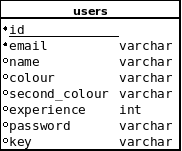
\includegraphics{Images/2/users}
\caption{The User record structure.}
\label{2_model_user}
\end{figure}

\textbf{Games} represent the decision for a group of people to play the game provided by the application. Games are created by filling out a form to establish some of its default values. Once a game is started many of its values are 'frozen' and cannot be changed. A game can be in one of the following stages: set up, playing, finished, or failed.
\begin{figure}[ht]
\centering
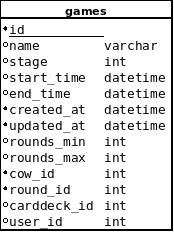
\includegraphics{Images/2/games}
\caption{The Game record structure.}
\label{2_model_game}
\end{figure}

\textbf{Cows} are representations of the condition of a cow. Each cow has five indications of this condition: welfare, body condition, level of pH in the rumen, amount of muck created, and the amount of absorbed oligos. These fluctuate as a consequence of player's actions.
\begin{figure}[ht]
\centering
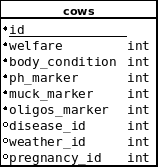
\includegraphics{Images/2/cows}
\caption{The Cow record structure.}
\label{2_model_cow}
\end{figure}

\textbf{Rounds} represent a period of time in a game. Within a round four phases happen, and every player has a turn. Each round an event happens.
\begin{figure}[ht]
\centering
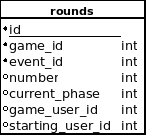
\includegraphics{Images/2/rounds}
\caption{The Round record structure.}
\label{2_model_round}
\end{figure}

\textbf{Cards} represent the deck of cards with a board game. There are two categories of cards: ingredients which can be used to create food rations, described below, and action cards. Action cards can be used once, changing some value of the game.
\begin{figure}[ht]
\centering
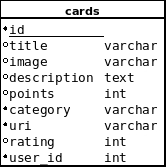
\includegraphics{Images/2/cards}
\caption{The Card record structure.}
\label{2_model_card}
\end{figure}

\textbf{Events} represent an occurrence that effects the cow in some way. One event happens each round. Three categories of event remain until replaced by another of the same category. These categories are: disease events, weather events and pregnancy. While active these events have on-going consequences.
\begin{figure}[ht]
\centering
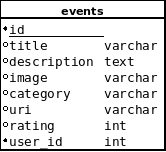
\includegraphics{Images/2/events}
\caption{The Event record structure.}
\label{2_model_event}
\end{figure}

\textbf{Rations} represent food rations, which are packages of ingredients. Once created they move through the digestive system of the cow until absorbed. When it is absorbed each ingredient gains a number of points.
\begin{figure}[ht]
\centering
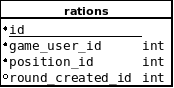
\includegraphics{Images/2/rations}
\caption{The Ration record structure.}
\label{2_model_ration}
\end{figure}

\textbf{Ingredients} represent types of food. They are created from an ingredient card and placed into food rations. Five types of ingredient exist: water, energy, protein, fibre and oligos. Each ingredient has advantages and disadvantages, and scores different points when absorbed by the cow as milk or meat.
\begin{figure}[ht]
\centering
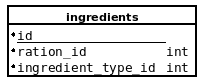
\includegraphics{Images/2/ingredients}
\caption{The Ingredient record structure.}
\label{2_model_ingredient}
\end{figure}

\textbf{Positions} represent places where players can move rations on the game board. There are 95 positions. Each position knows how it should be located by storing coordinates of it's location on the board. When a ration moves around the board, it gains a position, and uses the location provided by that position. As well as coordinates to define its location, a position has an area, corresponding to the section of the digestive system it is in. Every position has an order value, between 1 and 95.
\begin{figure}[ht]
\centering
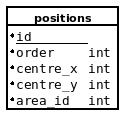
\includegraphics{Images/2/positions}
\caption{The Position record structure.}
\label{2_model_position}
\end{figure}

\textbf{Actions} and \textbf{Round Records} represent the history of a game. Each time a player moves a ration or uses a card an action may be created. These can then be shown as records of what a player has done during a round. In a similar way a round record is a snapshot of a value at a particular round of the game, because the value may later change.
\begin{figure}[ht]
\centering
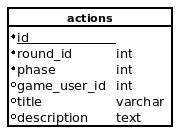
\includegraphics{Images/2/actions}
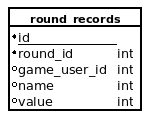
\includegraphics{Images/2/round_records}
\caption{The Action and Round Record record structure.}
\label{2_model_position}
\end{figure}


\subsection{Active Record Convention}
In the diagrams above, table names are in the plural form of the entity, and every entity has a unique id. Rails uses convention over configuration, so users must follow the designed conventions for data relationships to operate correctly.

Rails specifies that model classes will be pluralised, so the Game class will refer to a database record in the games table. Similarly, primary and foreign keys must follow convention. By default Rails uses a value named \textit{id} as a primary key. Foreign keys are the singular name of the record followed by \textit{\_id}, so a reference to a game would be \textit{game\_id} \cite{RailsActRec}.

This may seem restrictive, but during development, once the convention was understood and learned, it could be implemented many times with little effort. One advantage of these naming conventions is that once the table schemas are created, it is possible to automatically create relationships by simply specifying that the Games class has a relationship with Users. Foreign keys do not need to be specified, they are assigned automatically by following convention.

So relationships can be created in this way. The design also specified what the relationships between the main entities should be.

\subsection{Relationships}
A Database must be able to represent both records of objects and relationships between objects. Roughly a third of the tables in the final design of the database store such relationships. A diagram of the entire database exists in the appendix, but here it is worth considering one example of these relationships between Games, Users and Cards, seen in figure \ref{2_relationships}.

\begin{figure}[ht]
\centering
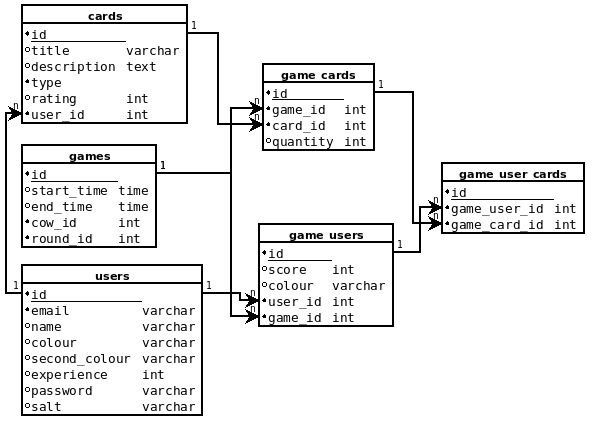
\includegraphics[width=6in]{Images/2/relationship_example}
\caption{The main entities are shown on the left. Tables creating relationships between them are shown on the right. These are known and 'joining tables'.}
\label{2_relationships}
\end{figure}

The game\_cards table is necessary because a many-to-many relationship is needed between games and cards. If players can choose which cards to include in a game, the game cannot blindly use any card. Also, quantities of cards are different within a game. Ingredient cards should appear much more often than action cards, so a quantity value is added in the relationship table. A card can also be used in many games.

The game\_users table is needed because another many-to-many relationship is needed between games and users. A user can play many games, and a game has more than one user. Also in this joining table is a score and colour value. The score is unique to the game user. A user has experience, but this is a different value form the score during a game. The game user colour value is used to store the user's colour during the game, this may be different from their usual colour if another user requires the same colour.

At this point a game has many cards and many users. But another relationship is needed. Users within a game (game users) also need cards. This will represent a user's hand within a game. The final joining table accomplishes this. It creates a relationship between game users and game cards. It is important that the relationship is between these two records and not between a game user and the cards table, as users could then have cards have not been chosen for that game.

The entities and relationships make up the database. Coupled with the server API, Rails can quite easily serve resources to the client with the minimum skeleton structure of models and controllers. Because of the innate structure Rails provides most of the logic of the server is just a thin covering enforcing permissions and rules on top of the relationships and objects established by the database. The server framework does include some complicated procedures, they will be discussed in the final section of this chapter, but these first two sections establish the majority of the logic of the game. 

Bringing the game together into a coherent and playable system is the work of the client side's user interface.

\section{The User Interface}
The design specification covered foundational aspects of the client side framework and user interface. This section includes first a description of the different pages needed for players to manage games and their details, and second a description of the game play environment.

\subsection{Pages}
Figure \ref{2_pages} shows all the conceived pages, and the links between them. The colours show which phase the page would be implemented in. The different phases are taken from the requirements specification: Phase 1 holds the core pages that are required for users to authenticate themselves, register and play a game. Phase 2 pages improve usability of the application, as players can change their details. Phase 3 allows crowd games, and a facility to provide a new password if users have forgotten it. Pages within the box require the user to be authenticated.

\begin{figure}[ht]
\centering
\includegraphics[width=6in]{Images/2/pages}
\caption{Pages are shown in different colours in order to show which phase of development they should be implemented in. The final phase, and some of the third were never created.}
\label{2_pages}
\end{figure}

Each page is not requested by an individual page request to the server. Instead the client side framework handles the load. An AngularJS routing plug-in \cite{AngularRoute} is used to map URLs onto Angular controllers and load the correct template by inserting the HTML into the DOM. This gives the feel of a standard application, but without the standard wait for pages to load.

The result of this is that once the index page is loaded from the server, all data received from the server is through the API, in JSON format.

A mock-up of each page was created. These helped to confirm the necessary navigation between pages, used to create the diagram above, and also aided the consideration of what data would be required for each page. The following descriptions are taken from the design specification.

\begin{figure}[ht]
\centering
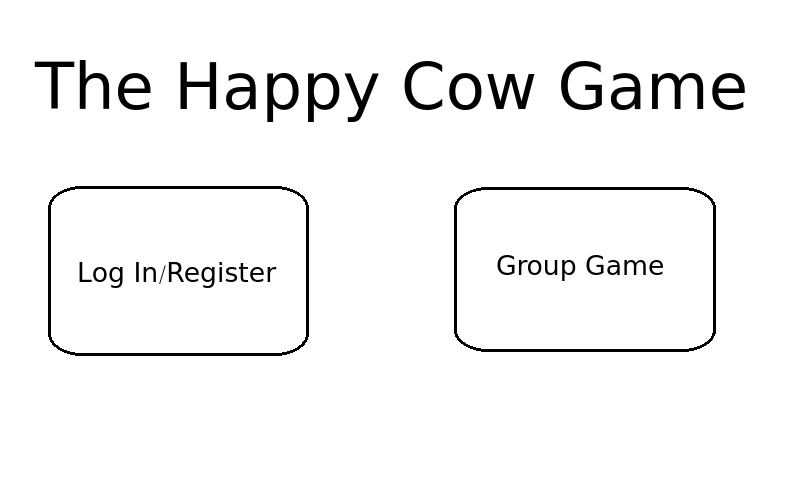
\includegraphics[width=4in]{Images/2/pages-1-welcome}
\caption{The Index Page.}
\label{2_page_index}
\end{figure}
Figure \ref{2_page_index} shows index page, the first page a user sees. It gives the options of logging in and registering, 
or creating a group game. A group game will only be possible in a later phase of development. 

\begin{figure}[ht]
\centering
\includegraphics[width=4in]{Images/2/pages-2-login}
\caption{The Login Page.}
\label{2_page_login}
\end{figure}
Figure \ref{2_page_login} shows the login page, which allows a user to authenticate themselves with their email and password. There is also an option to register, if the user is new to the site.

\begin{figure}[ht]
\centering
\includegraphics[width=4in]{Images/2/pages-3-register}
\caption{The Register Page.}
\label{2_page_register}
\end{figure}
Figure \ref{2_page_register} shows the register page. It is designed to look similar to the login page, but with a few more fields. This means that when choosing to register instead of logging in, the page updates and simply asks for a name and confirmation of the password as well. 

\begin{figure}[ht]
\centering
\includegraphics[width=4in]{Images/2/pages-4-games}
\caption{The Games List Page.}
\label{2_page_games}
\end{figure}
Figure \ref{2_page_games} shows the game list page, which is the entry point for games and other options available to a user. From 
here a user can see different games they are involved in, and a few details of each. Options 
allow a user to resume a game, or leave it if they don’t want to play any more. Other menu 
buttons allow a user to begin a game and view their profile.

\begin{figure}[ht]
\centering
\includegraphics[width=4in]{Images/2/pages-5-profile}
\caption{The Profile Page.}
\label{2_page_profile}
\end{figure}
Figure \ref{2_page_profile} shows the profile page, which allows a user to view and edit their personal details. The details needed to register 
are on the right. When updating a password or email, a confirmation email will be sent. The 
details on the right are to do with how users are represented in a game. 

\begin{figure}[ht]
\centering
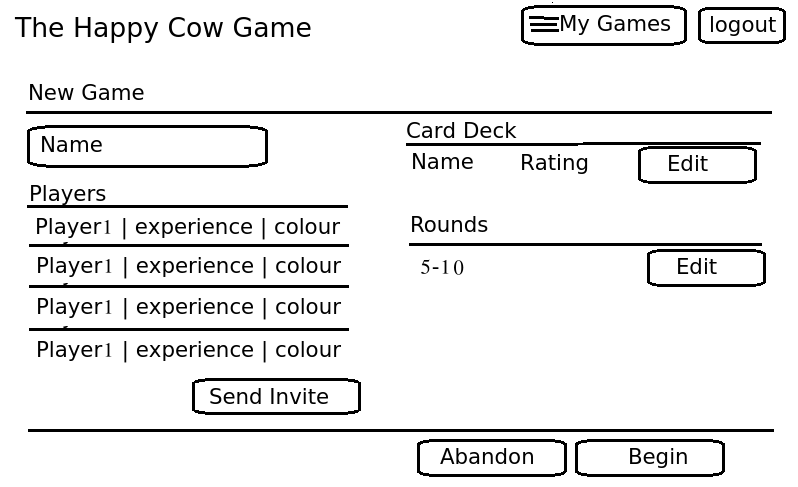
\includegraphics[width=4in]{Images/2/pages-6-new}
\caption{The Games Set Up Page.}
\label{2_page_setup}
\end{figure}
Figure \ref{2_page_setup} shows the game set up page. This page allows a user to create a new game. They can choose a name, a deck of cards to use, and the length of the game. They can also send invites to other players. At first these will be a link allowing a player to join a game themselves, but later if time allows, will be a message within the game. 

For players who aren’t creators but are joining a game, the edit buttons will not be available. 
The only action possible will be ’Join’ or ’Leave’.

\subsection{Game Play Environment}
The aim of the game play section of the design was to create a usable HTML mock-up that contained all the information needed to play the game without making the screen too cluttered or complicated. It succeeded in part, but once created and tested, many improvements were added. Those are explained later.

The original board, for the board game, contained the digestive system of the cow, and markers to record the cow's health and details. When playing the game, all the necessary information was visible by all players as they sat around the game.

\begin{figure}[ht]
\centering
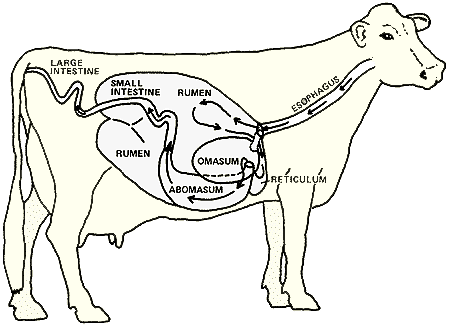
\includegraphics[width=6in]{Images/2/game-board}
\caption{The original game board. Players would sit around this and watch eachother move pieces. This is not possible with a web application where users can play accross a network.}
\label{2_play_board}
\end{figure}

When designing the user interface for the game play area, the aim was to keep these features, while also adding information about the current stage of the game (what round and turn it is), and a game menu. These details needed to be included, as they are remembered by players of a board game, but are more difficult to remember when playing a game online.

To organise the information that a user has to view and understand, three sections were created: a game information section, the current phase section, and a cow information section. These were laid out as shown in figure \ref{2_play_sections}. The purpose of each of these three sections is different, and so aims to compartmentalise the information it holds.

\begin{figure}[ht]
\centering
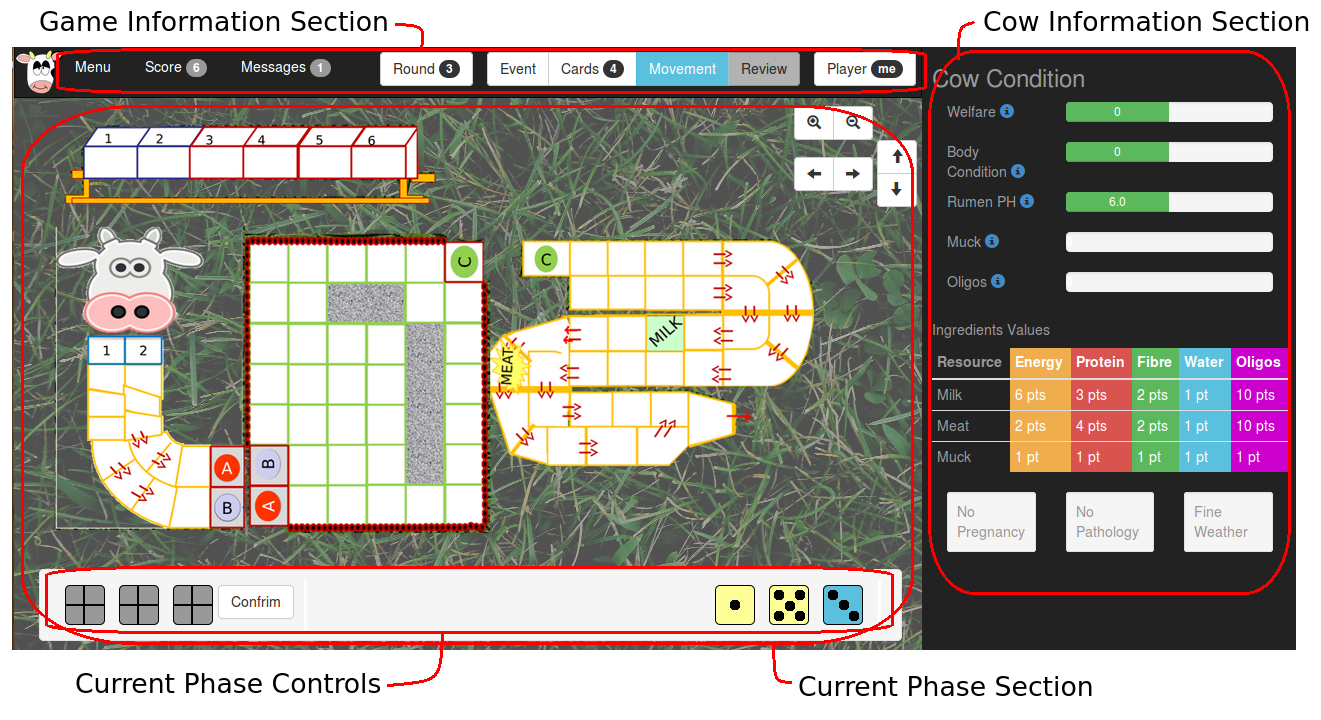
\includegraphics[width=6in]{Images/2/ui-sections}
\caption{This shows an early design of the user interface. There are three main sections: game information, cow information, and the current phase.}
\label{2_play_sections}
\end{figure}

Game Information provides information about the control and stage of the game. It is a menu bar, with buttons giving access to more options, such as details about player's scores and a history of the game. It gives a snapshot of the current stage of the game by stating what the round number is, by giving access to view the different phases within the round, and by showing the current active player (who's turn it is).

The Cow Information section keeps the crucial information about the cow in a static place. In the board game this information was on the board, where it can be easily seen by all. However, screens present a different scenario, one example is that they are limited in size. Fixing this information by the digestive system on a screen would make it much harder to find, and would probably involve scrolling back and forth. Instead it is fixed to the side of the screen, so it can be reviewed as the game progresses.

The two sections just mentioned provide information about the state of the game and cow. The Current Phase section contains the controls of the game. Players can select options, click buttons and drive the game forward by interacting with this section. There are four phases each round, so this section cycles through them in order, waiting for players to confirm choices before moving on to the next. The other two sections only react to changes that occur here.

The code that makes this all possible also needs to be organised. The Angular framework assigns controllers to the view by adding the controller name to an element of the DOM. All child elements are then within the scope of that controller. When the controller's data (model) changes, only the child elements within the controller will change. Controllers can be nested inside each other, and good practice suggests that each area of an application with a few controls has its own controller \cite{Angular}. This makes sure the code is adequately modulated.

Each of the sections identified above, therefore, was assigned a controller, and had a number of sub-controllers. Details of these are outlined in the design specification.

\section{Detailed Design Sections}
The design specification also considered two aspects of the application perceived to be complex, yet part of the core functionality: drawing and moving food rations, and ordering positions for pushing rations. Digging deeper into these two problems provided the outline of a solution, which helped plan the database structure and API of the application accordingly. By covering these sections in more detail the unknowns of the project were broken down into smaller problems, which could more easily be solved.

\subsection{Drawing and Moving Rations}
Food rations need a place on the screen, corresponding to their position in the cow's digestive system. On a physical board, rations would be moved from one square representing a position to another. On the screen however, the board is represented by a picture. In order to create the concept of a position a coordinate must be stored in the database. This was easily accomplished by creating the positions table, as described above. Each ration therefore has one and only one position, and the position defines where it should appear using x and y coordinates. See figure \ref{2_detail_coords}.

\begin{figure}[ht]
\centering
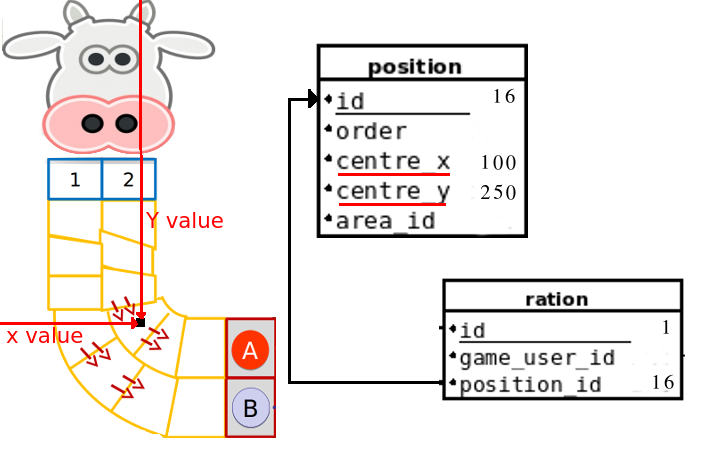
\includegraphics[width=6in]{Images/2/detail-1}
\caption{The original game board. Players would sit around this and watch eachother move pieces. This is not possible with a web application where users can play accross a network.}
\label{2_detail_coords}
\end{figure}

Using this structure food rations can be drawn on the screen, but that is only half the problem. Food rations also need to move through the digestive system. Users need to move rations from one position to another until they have used up their available moves. For this to be possible each position needs to know it's neighbour. An efficient way of accomplishing this is to use a graph data structure, as in figure .

\begin{figure}[ht]
\centering
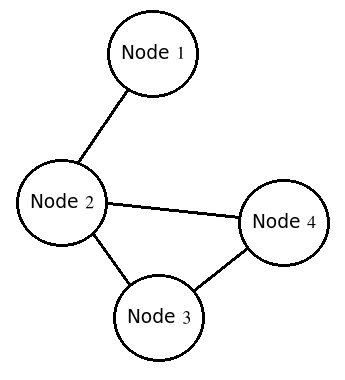
\includegraphics[width=2in]{Images/2/detail-graph}
\caption{A graph has a number of nodes, which represent positions, and links, which join positions. An example of a graph is a road map, where nodes are towns and links are the roads between them.}
\label{2_detail_graph}
\end{figure}

A graph is a collection of objects, each with a number of links. Each link connects two objects. In this case the objects are positions, with coordinates, and the links are values in a joining table. It is important that links are one-directional, as in the oesophagus and intestines rations can only move one way. To accomplish this, each link has a 'from' value and a 'to' value. When searching for neighbours of a position, only links with the 'from' value coming from the current position are valid neighbours. For bi-directional links, two links are needed pointing opposite directions.

\begin{figure}[ht]
\centering
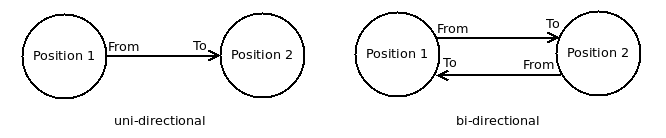
\includegraphics[width=5in]{Images/2/detail-links}
\caption{Two types of links are shown here. On the left is a uni-directional link, the graph cannot be traversed from position 2 to position 1. On the right is a bi-directional link, the graph can be traversed from either position to the other.}
\label{2_detail_links}
\end{figure}

To calculate the possible locations a food ration can reach in a certain number of moves, an algorithm is needed to traverse the graph. Starting with a position, the algorithm must visit all neighbouring positions and check the links of that next position. This is continued recursively until a depth of the number of moves given is reached. An example is given in figure \ref{2_detail_search}. 

\begin{figure}[ht]
\centering
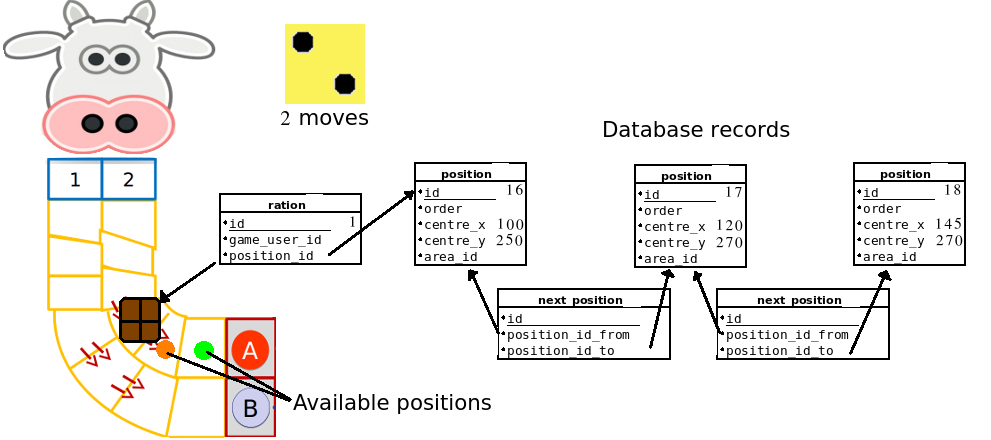
\includegraphics[width=6in]{Images/2/detail-2}
\caption{The ration is on position 16 and can move two spaces. So beginning with position 16, position 17 is checked, leading to position 18, where the algorithm finishes. If either of these positions had more than one link, the linked positions would also be added to the result.}
\label{2_detail_search}
\end{figure}

\subsection{Ordering Positions}
The second problem concerns the order of positions, there are a two reasons for positions to have an order. Some positions have a special significance. The trough is one example, as rations in the trough are automatically moved to the front until they enter the cow. Another example is the meat and milk positions. If a ration ends its moves on one of these two positions, it is absorbed, removed, and the owner is given points. Positions therefore need a number that is not the id, so that a few of them can be recognised by the system.

The second reason is for ordering rations as they are displayed to the player. It would be possible to use the graph to calculate the order of positions, however, this is computationally expensive. If each position has a number, which increases the further down the digestive system the ration is, this provides a way to order rations based on their position.

\begin{figure}[ht]
\centering
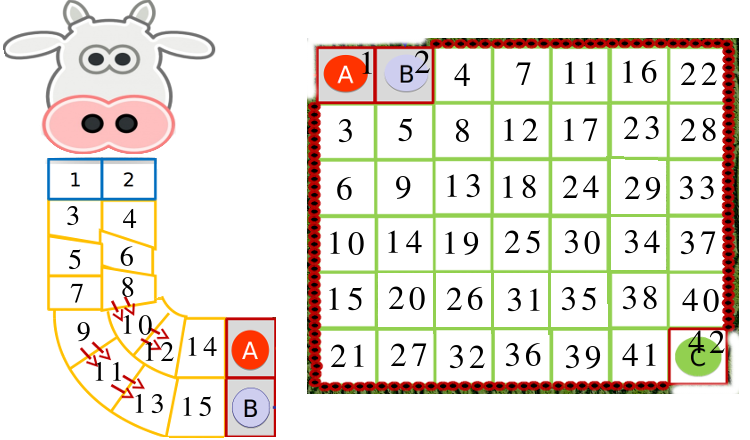
\includegraphics[width=6in]{Images/2/detail-3}
\caption{A proposed ordering of the positions within the rumen, in the inital design specification. This changed slightly during implementation.}
\label{2_detail_order}
\end{figure}

A further use of ordering positions was outlined in the design specification: calculating where a ration should land if it gets pushed from its position. The aim was to use the order to work out directions based on the difference between the order value of neighbouring positions. However, this was proven to be inaccurate and unnecessary. Positions already have reference to their location using x and y coordinates, therefore directions can be calculated with these values.

Both these problems proved more complicated than expected, therefore changing design as they were implemented. That will be explained in the following chapter, concerning the realisation of the design in the implementation of the project.
\chapter{Implementation}
An overview will consider the implementation of the project as a whole. Details of challenges and core parts of the system are then presented. The chapter will end with a summary of the requirements, and how they were met.

\section{Overview}
After finishing the design specification, work began on implementing the software. A project plan was drawn up, outlining a four stage approach to implementation:

\begin{enumerate}
	\item \textbf{Stage 1} Two weeks for a working prototype of the client side.
	\item \textbf{Stage 1} Three more weeks to build a fully working application of phase 1 (requirement specification).
	\item \textbf{Stage 1} Two weeks to implement phase 2, the usability requirements.
	\item \textbf{Stage 1} One week to make crowd games possible, phase 3 of the requirements.
\end{enumerate}

The first three stages became mixed, as their separation proved more of a hassle than benefit for reasons described below. Features were also advanced or postponed as their importance was re-considered. Below is a brief history of each of these stages.

Stage 1 was planned to be largely client side development. That meant adding the Angular framework to the HTML mock-ups created during the design. Its outcome would be a user interface complex enough to play a game, but only sitting on top of a dummy server API. After beginning development, it was soon apparent that some data needed to be persisted and updated by the server to properly create client software that communicated with it. Going out of the way to produce a solution on the client that would have to be replaced when the server logic was created was not worth the effort.

So stage 1 and stage 2 merged. Instead of focusing on a client/server split, development followed a core-feature-first approach. For example, players need to be able to see and use cards, so the user interface was created displaying cards with buttons to use them. Then the server was enhanced to allow users to use ingredient cards only, as these were needed to create rations. Discarding cards was deemed less important, and implemented later.

Stage 1 and 2 finished a week early, which allowed time for usability testing to begin. This generated feedback leading to more features and fixes. However, the next stage, stage 3, was concerned with implementing the usability requirements, making the game easier to learn and play. These new features and fixes therefore fitted in well, leading to significant improvement of the user interface.

As usability testing grew, larger groups needed to test the game. That meant each player having their own machine to play on became less practical, and so stage 4, concerned with crowd games was needed about the time it was planned. Stage 4 took less than a week to develop, yet required extensive testing. That, however, is the subject of the next chapter.

In the rest of this chapter particular parts of the implementation of the project that were challenging or interesting will be picked out and discussed.

\section{Working with AngularJS}
Development began with the client side. While Ruby on rails development was familiar as a framework, a disadvantage of using AngularJS was that it was a new technology. It presented a learning curve that had to be overcome. On the other hand, an advantage was the readily available plug-ins. Once understood, these cut down on development time. Early on in the project considerable time was taken finding good plug-ins, and then assessing their usability before proceeding too far with any of them.

\subsection{Bootstrap Library}
Bootstrap is a third party library famous for providing a quick and neat solution to common user interface demands. It provides templates for buttons, pop-ups, drop-downs, icons and text formatting. Traditionally, however, some of the more complex features of Bootstrap were powered by jQuery \cite{jQuery}, a popular Javascript library to allow easy DOM manipulation. However, Angualar has a different approach to jQuery. Insead of using jQuery-like DOM manipulation to change the view, the view references model data. Angular therefore does not blend well with jQuery. JQuery DOM manipulation in Angular controllers is overwritten when as the view will be quickly updated, and therefore should not be used \cite{AngularOverBB}. Instead, Angular plug-ins create their own solutions. Fortunately such a plug-in was provided which powered the usual Bootstrap features using Angular solutions, see \cite{AngularBootstrap} for details.

One such Bootstrap feature is the Bootstrap popover. Unfortunately HTML could not be inserted into the Angular-Boostrap solution. No way around this was suggested in the documentation for the plugin. Further more no solution seemed to be available, other developers must have accepted this inability or created their own solutions. 

Angular allows developers to create custom directives. In the Angular world, a directive is a view helper module which performs actions on the DOM. The popover feature was not complicated, and so the solution reached for this project was to create a custom popover feature that inserted an HTML template. By using a directive a combination of Angular and jQuery could be used to generate a working popover, called a 'popup'. The directive is detailed in Appendix E.

\subsection{Alerts}
Alerts are an important usability feature of the application, giving feedback about actions the users perform. If a button click is not allowed, an alert will be generated to inform the user why nothing happened. To create the alerts, the application began by using Bootstrap alert templates. This is a small coloured box with text that is dismissable. 

This worked for a while, but alerts are generated quite often, and it became apparent that they should wait for a set amount of time before fading away. This was fairly easy to implement. When created, each alert was given a lifetime in seconds. The Angular Bootstrap library provided alerts that could be dismissed in this way. However, like the popovers, these alerts could not hold HTML content, and so could not be styled.

The solution was to create a service. In Angular a service is a module of code that performs an operation, such as HTTP requests, sending emails, or in this case, creating and removing alerts. Within a service jQuery can be used to access and manipulate DOM objects. This solution used standard Bootstrap alerts, but also managed how long they remained. Another feature that could be added were batches of alerts. Some complicated server actions responded with a list of messages to display. The custom service checked if it was receiving a list, or a single message object and displayed them accordingly. The service is detailed in Appendix E.

\subsection{Restangular}
There are several Angular plug-ins that perform HTTP requests and handle the responses. The most basic is the \$http service, built into Angular itself. There are others, however, that are designed to work with RESTful API's, and provide short cuts for CRUD operations. Two of these were used, the Resource \cite{AngularResource} plug-in and Restangular \cite{Restangular}.

The first, Resource, seemed adequate. It enabled creating a service for each type of resource provided by the API. To query the resource, update or delete it, the service could be used, acting as a proxy to all requests to the server. For example, to request \textit{users/1}, a User service could be created with configuration set to access the \textit{users} route. It would map the get, update or delete functions to the correct resource route. This plug-in had one major shortcoming: it did not manage nested resources efficiently. To request users belonging to a game (\textit{games/1/users/1} with a RESTful API), a new GameUser service had to be created. Nested resources were key in the design of the server API, so another plug-in would be needed, if available, that could handle them.

The second plug-in, Restangular, did provide this support. Instead of treating every resource on the server as a service on the client side, it took a different approach. It provides a service from which any resource can be requested by using either a \textit{getList} method to request a collection, or a \textit{one} method with an id to request a single resource. These can be chained together to request nested resources. When a resource is returned, it is given the same attributes as the service. So while having the data of the resource provided by the API, it can also make the standard HTTP calls, thereby updating or deleting itself. This allowed a resource to be loaded and displayed to the user with little ground work.

It also meant that the client became much more dependent on the server and API. Very little data manipulation was needed by the client. When the model changed, a resource loaded could simply be updated by a patch request to the server, and then performing a get request to re-load it. This lead to the merger of stage 1 and 2 during development, already mentioned above.
	
\subsection{Storage and Security}
Another plug-in was used for client side storage. Storage is used to provide a session for the user. This is because the server API should be stateless, yet to protect user's security, authorisation is needed to access and update almost all resources. The best way to accomplish this is to require a user id and key in the header of all HTTP requests \cite{APISecurity}. Without these details requests will be returned with a 401, unauthorised, status.

So how does the user provide these details in the header? A login action, within the users controller, is outside the authentication check. This action checks the given user name and password, and if they match, returns the user details with an access token included. That access token is then used to validate user requests until they next login. Using an access token is a secure way of requesting a secret key that does not require the user to send their password with each request.

All actions on the server, but for login and registration, therefore have an associated user. That user can be checked against the information being requested, or updated, to verify that they have permission to access or amend the data. If a request is updating a user, game user, game user card's or a food ration, the ownership of the object can be checked. If users are updating game details, the system can check if they are the owner, if the request is ending the current turn, the system can check if it is in fact the authenticated user's turn. All this can be done without a session, simply with a user ID and secret token. Implementing this type of security is known method outlined for RESTful applications \cite{APISecurity}. The solution used is detailed in Appendix E.

Coming back to storage, it is therefore used to hold user details, including the access token, on the client side. This means that a session is maintained in the client without the server needing to know about it. There are two types of client side storage, session storage and local storage \cite{ClientStorage}. Both allow an application to store data in the web browser between page requests, making sessions easier and smoother to manage. Local storage is a persistent version of session storage, available to any tab and accessible forever, unless deleted by the application. There is a 5MB limit on storage per application. This is imposed by the browser.

Using the ngStorage plug-in \cite{reference}, either types of storage can be accessed simply by writing values to a provided storage object. An application prefix can be added, so that all data stored is a child of the application place holder. This mitigates the risk of other applications using the same storage key and wiping out the user's session. Session storage was used for this project, so that if users restart their browser, they do not continue to be logged in. It was a useful plug-in that worked as expected and saved a lot of hassle converting values to and from string types as they are stored and retrieved.

\section{Positions, and their Complexity}
As explained in the previous chapter, the game board is represented on the screen as a single image. In order to move food rations around, locations are identified by coordinates stored in the database as positions. A food ration therefore has a single location, allowing it to be positioned on the screen. 

When a player wants to move a food ration from one position to another, available positions must be highlighted, from which the user can choose one. Within the database, positions have the structure of a graph, with nodes and links between. To search for all the available positions the graph must be traversed up to a prescribed depth, and the response returned to the client.

\subsection{A Recursive Search}
The first attempt at traversing this graph took a recursive approach. A tree was constructed, using the starting node as the root, each link was followed and added to the tree. The tree was then encoded as JSON, sent to the client, and all it's positions rendered on the screen.

\begin{figure}[h]
\centering
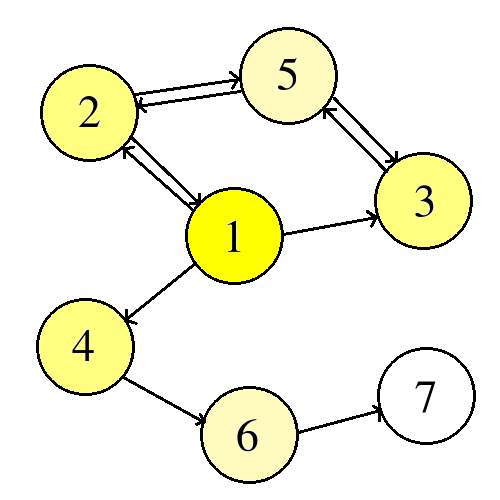
\includegraphics[width=2in]{Images/3/graph}
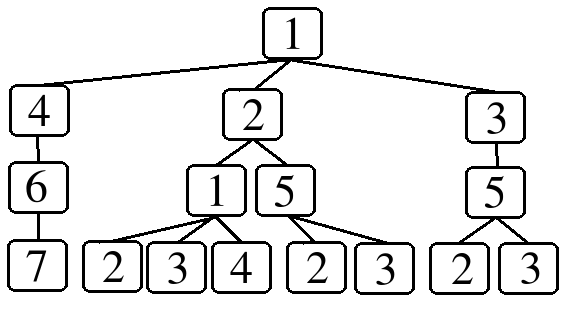
\includegraphics[width=2.5in]{Images/3/tree-1}
\caption{On the left is a visual representation of the arrangement of seven positions as a graph. On the right is a diagram of the result of a traversal on such a graph. Beginning at position 1, each link between nodes is followed until 3 steps (a depth of 3) have been taken. This tree would then be sent to the client, and each position drawn in place.}
\label{3_recursive_search}
\end{figure}

Unexpected and negative results quickly became apparent. The first and last positions were shown in a different colour, but did not appear where expected. This was due to the recursive traversal and display of the tree. Because some positions had two links between them, in opposite directions, the traversal could end up in a loop, or doubling back on itself. All the possible routes through the tree were being displayed, but this meant that when a neighbouring position was selected, the route to it may have gone through several other positions to get there.

\begin{figure}[h]
\centering
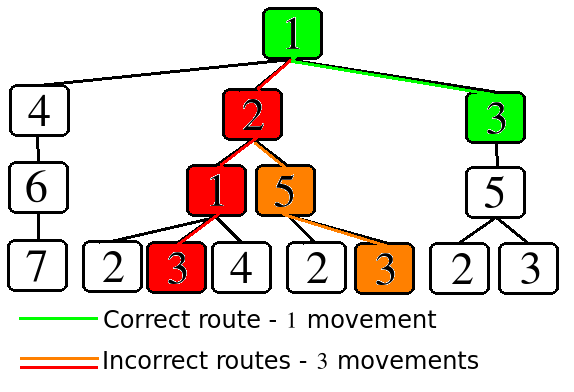
\includegraphics[width=3in]{Images/3/tree-1-example-1}
\caption{This shows how a tree was drawn by the client. No order was given for drawing, so starting with position 1, the right-most link was followed (order). Therefore positions to the right of the tree were hidden by the same positions drawn after. The position that should have been drawn first is shown in green, yet the incorrect routes, shown in red which take more movements, were shown.}
\label{3_recursive_search_wrong}
\end{figure}

If the problem involves positions occurring too many times, the first solution seemed to be checking if a position had been previously rendered, and if so, excluding it from the search. This was done on the server, but had even less usable results. Instead of showing all positions in the tree, only the first positions in the tree traversed were shown, but instead of improving the positions displayed, it introduced 'garden paths', where a random and unhelpful series of positions was chosen, this in turn created dead-ends and unreachable positions.

\begin{figure}[h]
\centering
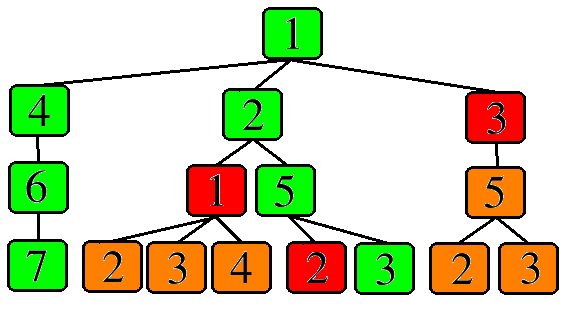
\includegraphics[width=3in]{Images/3/tree-1-example-2}
\caption{Positions in green are reached, positions in red are excluded because they have already been included. Positions in orange are not displayed because their parents are excluded. Once again, the shortest route to position 3 is not taken.}
\label{3_recursive_exclude_wrong}
\end{figure}

The problem lay with the recursive approach. To solve this, the graph had to be traversed in a different way.

\subsection{Traversing in Levels}
Instead of assembling the tree by following all possible paths until a certain depth, the tree must be built up in levels. The root node is added to a list of positions to display, and then all the positions it links to are added to the next level to check. When checking this level, if a position has not already been included, it is added to the list of positions to display and positions it links to are added to the next level to check. This continues until the specified depth is reached.

\begin{figure}[h]
\centering
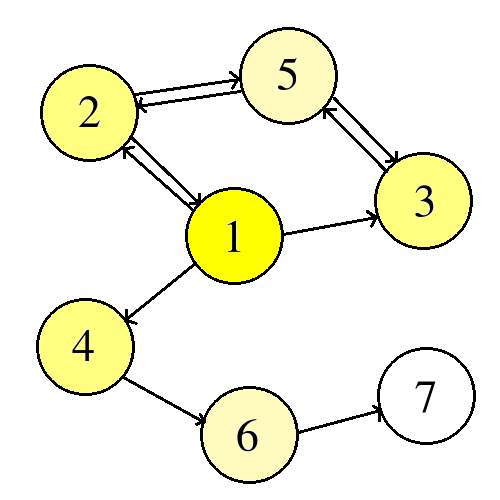
\includegraphics[width=2in]{Images/3/graph}
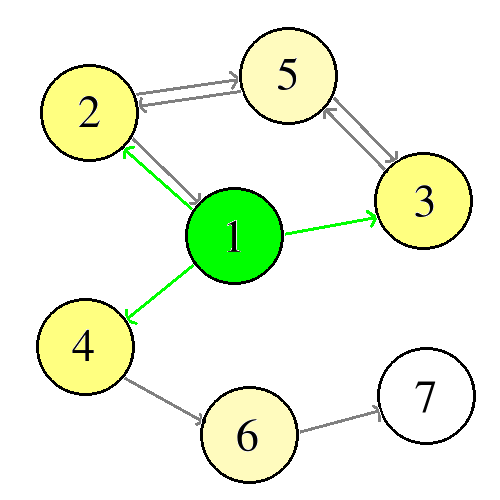
\includegraphics[width=2in]{Images/3/tree-2-step-1}
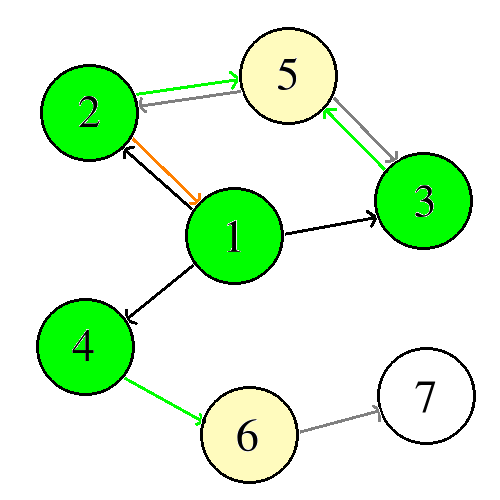
\includegraphics[width=2in]{Images/3/tree-2-step-2}
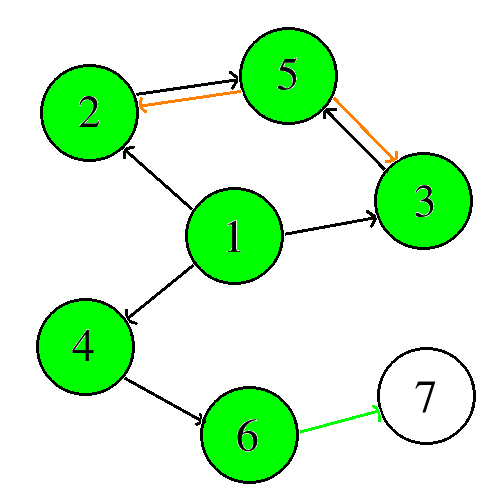
\includegraphics[width=2in]{Images/3/tree-2-step-3}
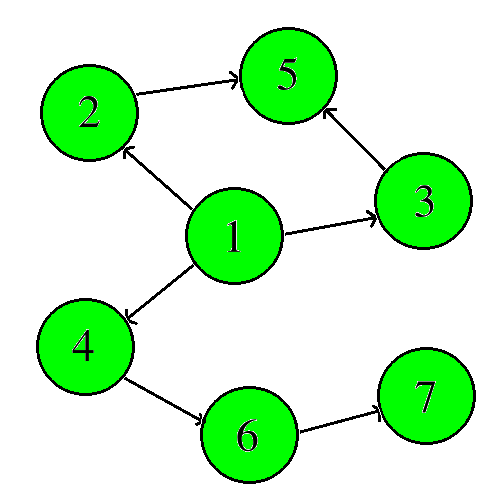
\includegraphics[width=2in]{Images/3/tree-2-step-4}
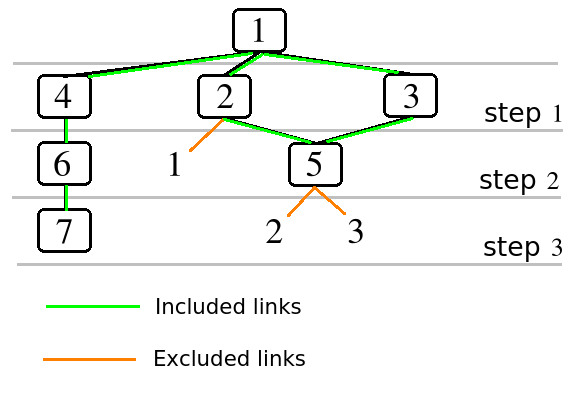
\includegraphics[width=2in]{Images/3/tree-2-full}
\caption{Steps of traversing the example graph, one set of links at a time. The resulting tree is shown at the end.}
\label{3_levels}
\end{figure}

This was implemented on the client. The server returned a recursively built tree, these were the allowed positions. The client built these into a graph, and then traversed the graph in the manner described above to render them. 

As a solution it worked, positions were displayed correctly, and it is still the method used by the system. However, there were several more improvements to make. Most notably, with a depth of ten or more, building a tree on the server and then constructing a graph on the client and traversing it took some time. It was too inefficient.

\subsection{Improving Efficiency}
The inefficiency was due to the traversal algorithm undergoing several changes. By this point the server was traversing the graph to find all the possible positions. These positions were being sent to the client where the graph was built and then traversed in the correct method described above. When a large depth was required, this could take some time to render. Latency in displaying the positions was due to the recursive method still being used on the server. Many positions appeared in the tree multiple times, the larger the depth, the more often they were included. Both the time it took for the server to build the tree, and send a gigantic package of JSON could add minutes to the process.

\begin{figure}[h]
\centering
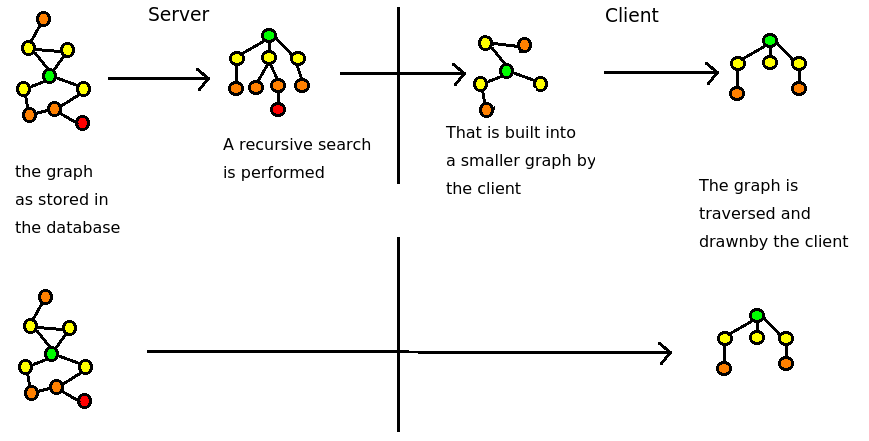
\includegraphics[width=5in]{Images/3/efficient-example}
\caption{The inefficient, previous method is shown above. The method below shows the change, which made rendering positions much faster. The most expensive step was building a recursive tree of possible positions. Consider a block of positions, each with four links. This can quickly create a maze of possible solutions. The recursively built tree tried to represent every route, whereas a tree built in layers merely presented an allowed subsection of the graph.}
\label{3_efficient}
\end{figure}

The solution was to remove an extra traversal and build step, shown in figure \ref{3_efficient}. Differences in speed were huge. The new solution experienced hardly any waiting time, compared to several seconds or minutes previously.

\subsection{Checking for Obstacles}
The task of rendering positions was complete. A further advantage, however, of moving the traversal to the server is worth considering. It was the ability to check the movement of food rations. A food ration can move a number of positions in a turn. To begin with, all movements were made by the client, and when finished the server was updated with the final position. Other elements in the digestive system become obstacles for food rations. 

Rather than relying on the client to recognise these objects, and prevent users clicking to move their ration on those positions, the checks could now be performed on the server. Clients are much more malleable and their restrictions are easily circumnavigated. While it is unlikely that someone would hack this application in order to cheat, best practice requires the server to validate user actions without relying on the client's suggestions \cite{APISecurity}.

A requirement, based on the original rules of the game, made avoiding obstacles more complicated. Food rations cannot normally move over each other, they provide obstacles for other rations. If, however, one ration has more fibre ingredients than another it may push past another ration. With checks implemented on the server, obstacles in the shape of food rations could be compared to the food ration on the root position. If they have less fibre ingredients, then they are no longer considered obstacles.

Delving to this depth into the display of positions was an aspect of the project that had not been considered during the design phase. It proved a challenging, yet rewarding, puzzle in which the benefits of different ways of traversing a graph were explored. The final algorithm for traversing the graph of positions is detailed in Appendix E.

\section{Card and Event Actions}
Cards specifying actions for the players to carry out are often used in board games. When such a card is played, it is usually trivial to carry that action out. To build the same rules into an application, however, is a different matter. Especially if the cards require further user input.

\subsection{Complex Specific Actions}
Both cards that players hold in their hand, and events which happen at the start of each round include actions. Some examples from the board game are:
\begin{itemize}
	\item \textit{'Move the pH marker up or down 1 to 3 squares, your choice.'} That seems simple, but how does the application query the user's choice? A form is needed where the user can specify whether they want the marker to move up or down, and one, two or three places. With the form comes the need for a special server action to process the results.
	\item \textit{'Change up to two ingredients of any player's food ration by the same number from your hand.'} This is more complex still. It requires first a form where a user picks a food ration, and then one or two ingredients. The player must then be presented with a choice of ingredients to discard, up to the same number.
	\item \textit{'All rations that leave the rumen this turn have up to one fibre ingredient turned into protein.'}  This does not require user input, but it does need a way of recording that the card has been played in a round, and to check each ration that moves past a certain position. That means an extra value, or record in the database just for a card action.
\end{itemize}
	
Some actions were easier, involving moving a few values of a cow record up or down, or changing a player's score. These were implemented by performing an action based on the type of card when the request comes to the server for it to be used. The rest of the actions had to be simplified, so that they did not require user input, and could be completed in the scope of the project.

\subsection{Cow Events}
As well as one off actions, some events cause an ongoing effect. These are categorised as weather, disease or pregnancy events. In each of these cases the event remains active until it is replaced by another event. For example, a weather event such as 'Hot Weather' remains active. This is achieved by setting a value in the cow record called 'weather\_event' to the id of the event. That is strait forward, the difficult part is making sure its action is carried out. It must be performed whenever relevant while the event remains.

To do this, each persistent event was given a helper method in the cow model. The method returns a boolean value, indicating whether the event is active. Throughout the code base, these methods can give an indication of the state of the cow, while keeping in one place the logic to check if the event is active. An example is constipation or diarrhea in the intestines of the cow. When deciding how far a food ration can move, a test is needed to see if either of these diseases are active. If so a further check is carried out to test whether the ration is in the intestines. If so, its movement is affected.

Having considered server functionality, the client interface also took a large section of implementation time. Aspects of it are well worth discussing.

\section{Updating The Client}
Beyond the plug-ins and learning curve provided by the client side framework, a feature of note not covered by the design, yet needing implementation was updating the client.

Synchronising the client and server was not covered in the design. As the server is stateless, all the initiative comes from the client. It is the client that requests data. The server merely processes a request and returns a result. Most of the time this is all that is needed.

However, when several people are performing actions on the same data within an application, updating every client with the latest data goes outside of the normal work-flow described above. This regularly happens within the application. As players take their turn, the data will change, and when they finish their turn, the server is updated and registers that it is the next player's turn. However, the next player's client will not be updated automatically. They will not know it is their turn without refreshing the page.

The issue lies with server-to-client communication. There are three potential solutions. It was a matter picking the simplest one that met the needs of the project.
\begin{itemize}
	\item One solution is for the server to somehow push an update whenever the state of certain objects change. This is possible between servers, but breaks the standards of client-server requests and is therefore unsupported. When searching for a way to implement this within the Rails framework, no documentation for an approach could be found within the Rails community. This suggested it is not a common approach.

	\item The second solution is for the client to perform a request, which the server holds until a change is triggered in an object. When that happens it returns the request with the updated data. The client can then update and perform another request. There is little support for this in Rails or Angular however.

	\item The third solution, which was implemented, was a regular update loop. When a game started, the client is set to perform a request every five seconds. This is a long enough wait to avoid over loading the server, yet is a natural enough period to wait for a page to change, based on some event.
\end{itemize}

With this in place, players can play games across a network without refreshing the page once.

\section{Crowd Games}
Phase three of the requirements analysis covered crowd games. They are games where players take turns to perform actions at one client, instead of playing across a network using multiple clients. Challenges were perceived when it came to implementing this new dynamic, but in event it was not too arduous a task.

\subsection{Designing for Crowd Games}
As crowd games were always in the list of requirements, they were built into the design of the user interface. 

The biggest question was how to securely manage accounts when many players needed to be logged in at once. It was planned that when creating a crowd game, the set up page would require a user to log in before they could join. This prevents a user being added to a game without their permission.

When users login, their details are stored in an object in the base controller, from which all other controllers extend. Every time the authenticated user's details were used during implementation, they were sourced from this object. When a user logs out, the details of this object are erased. This design helped to keep the concerns of user authentication in one place.

\subsection{Changing Accounts}
When it came time to implement crowd games, properly authenticating and changing between users was simple. When the game is created users authenticate themselves. These details are kept in local storage as a list of users who are playing the game. When a player ends their turn, the id of the next player is returned by the server. The list of players is searched for that id, and the player is authenticated and their details fetched.
	
\subsection{Changing User Authentication}
Once crowd and single games were implemented, a cleaner design was conceived with two types of user account that could be authenticated. It became necessary to separate the account within a game, from the account of a player who had logged in to view their games. This was because, when playing a crowd game, a player could return to the main menu, and the authenticated player would be the player whose turn it currently is in the crowd game.

To avoid players being logged in through a crowd game, a user was defined as someone who authenticated themselves to view information, such as their list of games or profile. Whereas a player was the person currently authenticated and taking their turn in the game. In a networked game, when a user resumes a game, they become the player as well. The player account can be changed without affecting the user who is logged in. This helped simplify management of accounts in crowd games.

With this separation of accounts the possibility arose to remove the distinction between games altogether. When a game is begun players could choose to login on the same machine, or take a networked approach, the game could then either automatically log the player in, or wait for them to take their turn, if they have not authenticated themselves.

This unification of game types actually simplified the process of setting up games had a threefold advantage. First of all, instead of asking a player to choose between two types of games, and explaining the differences, game creators merely have to define players as being at the same machine as them, or distant across a network. Users can begin a game across a network, but resume it later, together at the same machine. 

The second benefit is that there was no real difference between networked and crowd games, but their set up. By combining the games the set up pages of crowd games could be removed. Any future changes did not have to be replicated across two types of set up page.

The final benefit was that by making the games operate in the same way many of the issues of distinguishing between crowd or networked games in the code were removed, making the code simpler. This was already done by the system, but it also had to work out what type of game was being played, and unnecessary burden. The flexibility of assigning users as distant or present more naturally fitted the design of the system.
\chapter{Testing}

Testing is an important aspect of any project. Even small projects can benefit from automated test to quickly check if a change has created an error somewhere in the code base. The larger a project is, the more fundamental testing becomes.

Three types of tests were outlined for this project in the requirements specification, unit tests, functional or end-to-end tests, and usability testing which included testing the application using different browsers. First testing within the server application will be considered, then tests necessary for the client side of the application will be explained.

\section{Server/API Tests}
The server provides the game logic, and resource API necessary for the game. Therefore, testing the server's functionality means making sure the API serves resources as expected and that the game logic responds as designed. Rails provides two types of tests that fit these needs: functional tests and unit tests respectively.

\subsection{Unit Tests}
The Rails framework provides model classes, each representing a type of record stored in the database. For example, the details of an application user will be stored as a record in the database, and so a User class  can be used to interact with the record and provide methods common to all users. Unit tests help to test each of these models in separation from the rest of the application in order to determine that its methods act as designed.

Unit testing began before the testing phase of the project was due to start. This was because as the application grew in complexity it became increasingly hard to check that areas of the application responded as intended. Unit tests helped to confirm that they did, or did not. So rather than being something tagged onto the end of the project, these tests actually served a useful role during development.

All models of the application have a respective unit test. Some of these are quite basic, because records that join two other tables may not require any logic of their own. In this case the tests establish that the joins between tables are set up correctly. Other test classes are extensive. In order to make the server application modular and to adhere to DRY (Don't Repeat Yourself) principals, as well as to make it more easily testable, much of the game logic was moved from the controller classes to the model classes. Some classes such as those representing games, cows, moves and cards had to test large blocks of logic requiring between ten and twenty tests each.
	
Two aspects of unit testing are worth a particular mention, as they involved learning new techniques. These are fixtures, and seeding random number generation.

Fixtures are a technology employed by Rails for quickly generating test data. A test database is used for test. This is emptied and loaded before each series of tests in order to ensure that tests are not disturbed by the results of other tests. Fixtures are a YML (Y.. Markup Language) representation of data that is loaded into the test database before running each test. So fixtures provide the 'truth' which tests are validated against.

This means that test data can be created quickly. However, certain relationships proved difficult to replicate using these fixtures. The positions that make up the board are stored in the database. In order to test the movement of rations, both the positions, and the joining records making the links between positions need to be supplied using fixtures. This type of one way relationship between records of the same table could not be done using fixtures, so while test positions were generated, none of them were connected to each other in the way necessary to build the board. Instead, positions had to be joined within the logic of the tests, before a test was carried out.

The second aspect that made testing more of a challenge was random number generation. The best example is dice rolls. When moving a food ration a user is presented with some randomly generated numbers between 1 and 6 to represent the roll of a dice. But how could this random generation be tested? Each time the dice rolls are generated they have a different result, by design, but tests need to know what their expected outcome is in order to test that the numbers have been generated as expected.

The solution was seeding the random number generator. Rails provides an easy method of doing this, and using a set-up utility before each test, the random number generator could be seeded so that it always gave the same result. Tests could then be built using these results.

So tests for all the application models were created, and application logic was updated until the tests representing the game requirements, passed. A full list of unit tests can be found in Appendix D.

\subsection{Functional Tests}
With the model logic working as expected, another important aspect of the server framework is the controllers, which serve the requests coming through the API. Controllers use the data models, but build on top of them, often adding an extra layer of functionality, or combination of model calls. This functionality needs testing. Because the API is stateless, and there is no particular order in which the API needs to respond, these serve as functional and integration tests.

An important aspect of these tests involved ensuring that unauthenticated users were denied the ability to access or amend resources that do not belong to them. This was not as straightforward as expected, because in order for game objects to be represented, a user may need read permission on another user's food ration, but should not be able to make changes to it. Different methods of authentication were therefore needed for GET requests than POST, PATCH and DELETE requests. This was achieved by testing that the user was authenticated or that the user was a player of a game for most GET requests. For most POST, PATCH and DELETE requests the controller checked that the user was the owner of the resource.

All the possible requests that can be made through the API were tested using functional tests. This helped to uncover some flaws in the API not considered in the design. One example is updating a player's moves. Ther controller checked for a parameter which indicates if the dice should be set. This was performed on the condition that a food ration had been chosen, but the controller did not check if the dice had been previously set. By creating tests, this small error was noticed and could be changed.

Functional testing also initiated the creation of standard responses for resources that were not found, or for unauthenticated requests. So the controller level of the application benefited from testing by becoming more uniform and having some lose ends removed. A full list of functional tests can be found in Appendix D.

\section{User Interface Tests}
Usability testing, from the beginning of the project, has been perceived as a vital part of the development of the application. This section explains how these tests progressed, and some of the benefits of performing them. Then automated client tests are considered.

\subsection{Usability Testing}
Usability testing began as soon as the project was in a state where a game could be played. Five groups of users helped to test the application in seven meetings held over a month. These comprised friends, family, computer science students, and the project client and supervisor. An attempt was made to get biologys students, one target audience, to test the game in a lecture setting, but no interest was shown. Despite this, the meetings held were extremely helpful, generating many suggestions.

To begin with players were registered by being entered into the database so that feedback could begin before registration was implemented. Some suggestions by users were put to effect straight away, if they were simple and fit with the current section of the project under development. Other suggestions were noted to be added later. Fixes that prevented the game being played were addressed as soon as possible.

Much of the feedback from users picked out logical flaws or bugs. These will not be focused on here, but are detailed, along with solutions, in Appendix D. It is more important to consider how user feedback impacted the overall design of the project and led to significant changes in the way the application data was presented.

Despite the time taken to create a good user interface design during the design phase of the project, the user interface needed many improvements. When users first tested the application, the main theme of their feedback was that controls were too complicated, and the game too difficult to pick up and play without knowing the rules before hand.

The aim of the project was to make a game that anyone can play. However, this goes beyond representing the existing board game as simply as possible. When playing a board game people expect to have to read a set of rules. Users of a web application, however, want to be able to pick up the rules as they go along. So not only do the controls need to be easy to find, but at the same time their location also needs to suggest how they are used, so that users do not have to read about how to make use of them.

User feedback, in Appendix D, suggested the best way to do this was to present only one task for the user to work on at a time. Instead of giving the user a page with many controls, let one action follow on from the other, with one decision to make at a time, while also making the impact of that decision obvious.

An example of the difficulties users had with understanding the controls is one person who missed the point of the game entirely when testing it. Because of a lack of information about how to play the game, this user clicked on buttons to finish various phases without once creating a food ration. So the game never presented the option of moving a food ration. As a short term solution a page of instructions was created explaining how to play the game.

A better solution was needed, however, for the game to fit its requirements of being easily playable in a classroom. A new user interface design was created based on user feedback and the one-task-at-a-time principal described above. This design had three main objectives that led to it's changes. 

The first concerned the fact that users found it difficult to associate the phase control buttons with the different screens that were displayed during a round. This is because unless the phases of the game are known, the names of the buttons referring to different phases were quite obscure. To avoid this confusion, cards and the cow digestive system can be shown on the same screen as shown in the diagram [reference]. This means that different phase screens are not needed. A user always has the same main view.

The second objective is to provide one task at a time. This is done by having just one command or question for the user to respond to at a time, and in a recognised place. While the first objective places all the information on one screen to view, this second objective prevents confusion from this information by focusing the user's attention to one place.

\begin{figure}[h]
\centering
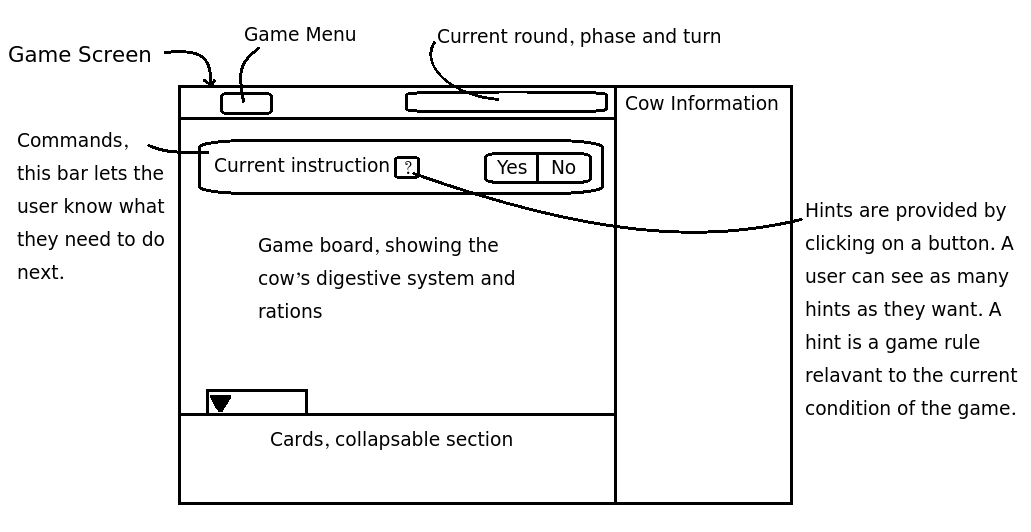
\includegraphics[width=3in]{Images/4/new-design}
\caption{A new proposed design, based on user feedback.}
\label{4_new_design}
\end{figure}

While the first two objectives focused on getting the user through the stages of the game, the third objective of the new design was to provide optional hints about some strategies a player could use as they make decisions during the game. This was planned in the form of a 'hints button'. Players could use this button as a way of asking for advice about what to do. The advice would depend, to some degree, on the current state of the game and the user's available cards.

\begin{figure}[h]
\centering
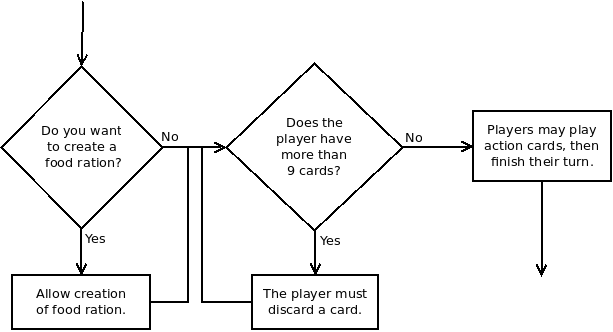
\includegraphics[width=6in]{Images/4/command-stages-cards}
\caption{The cards phase was broken up into these five stages. These stages are designed to improve usability, as a player will only have one task to perform at a time.}
\label{4_cards_commands}
\end{figure}

\begin{figure}[h]
\centering
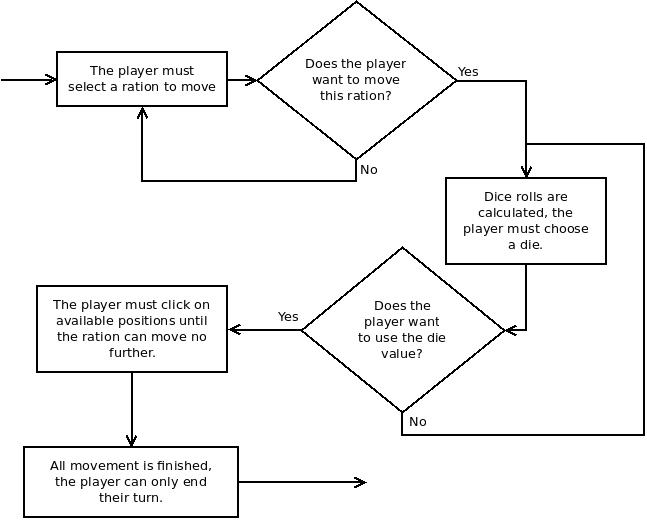
\includegraphics[width=3in]{Images/4/command-stages-movement}
\caption{The movement phase was broken up into these six stages. First they must choose and confirm a food ration, then they are presented with dice, and must move a food ration the number of positions shown on the dice they select.}
\label{4_cards_commands}
\end{figure}

Due to time constraints, only one objective of the new design were implemented: the second, single tasks at a time. This split the two main phases, the cards phase and the movement phase, into several sections, described in the diagrams below.

\subsection{Automated Testing}
On the client side automated testing is made possible through technologies such as Jasmine and Karma \cite{KarmaJasmine}. However, testing the client for the purposes of sifting the code base for bugs was not a priority of the project, as it had already been accomplished by the usability testing explained above. For maintenance, end-to-end testing would have been useful, but due to time constraints it was not included.

\subsubsection{Unit Testing}
AngularJS is modularised, making unit testing possible, and a good amount of documentation exists on how to begin. However, each module implemented for the project relied heavily on data returned from the API. Client side unit tests do not work well with asynchronous HTTP requests, because they require a stubbed service to be implemented that can respond instead of the server. As the modules of the project were thin layers dealing with the display of data returned from the server, any unit tests created would actually be testing the stubbed server API instead of the application, and so were not worth the time to create. 

\subsubsection{End-to-end Testing}
Instead of testing the data in separate modules, end-to-end testing attempts to mimic common uses of an application. If implemented these could be useful for maintenance of the code, as a way to ascertain if the functionality of the project remains the same after a significant code change. However, usability tests uncovered most issues that detailed tests would pick up, and so, with time constraints, these tests were left not implemented.
\chapter{Discussion and Conclusion}
This chapter presents an evaluation of the entire project, considering what worked well during the process of design, development and testing, and how that process could be improved. A summary of enhancements is then given. These are less vital parts of the project that could not be implemented due to time constraints. Finally a conclusion summarises this report.

\section{Critical Evaluation and Insight}
It is frustrating when there is so much that could be done within a project, but time constraints mean that useful sections are left out. That is certainly true for this project, yet looking back much has been accomplished in the last thirteen weeks. The happy cow board game is playable as a web application. Players can register and manage their games. The user interface design has seen numerous improvements, becoming more robust with each change. Having worked hard to make this much possible, there is a natural desire to see the project grow, and to explore all the possible ways it could improve.

Such ideas for improvement, and how the project could have developed had more time been available, are considered in the next section. Here the topic of discussion is what has been accomplished, and how well it has been done.

\subsection{The Process and Method}
Detailed requirement specification, up front design, and weekly meetings with the client have all greatly helped shape this project and guide it to maturity. The process was a delicate balance of some plan based structure with frequent meetings to assess the progress of the project. This resulted from taking the core elements of a plan based process, with continued client input to keep the project on track.

In the early stages of the project, weekly meetings with the client helped me to check the requirements and design. At this stage the project was more strictly plan based and focused on documentation.

The requirements analysis began with turning the existing game rules into a list of tasks, and adding to these necessary application tasks. When reviewing the tasks it was decided there was not time to complete all of them, so they were organised into four phases. The requirements helped to clarify game rules and provided a good check-list to gauge progress.

Building on top of the requirements, the design drilled down into the unknown of the project to set some rules, and break down the problem into smaller sections. Its purpose was not to be detailed to the degree that it provided a code skeleton that needed to be merely filled in, but to make sure that no area of the project remained 'in the dark'. The database and API design in particular were invaluable as the project went forward. Bits were added, but the existing structure was only slightly changed. The design was not needed for communicating between teams of developers, yet it was a useful planning tool, and a reference. The good guidelines it provided meant that development could begin more quickly, and ensured that the foundations of the project had been well considered.

As the design stabilised and development got under way, meetings turned into progress checks and usability tests. A number of meetings helped create a list of bugs to fix and things to change where requirements were misunderstood. These meetings also helped to prioritise tasks. At the beginning of the week we would agree what tasks in the current three week development phase needed to be done first. At the end of the week we would review them. This methodology has practices of Scrum, with retrospectives and sprint reviews. At the time it was simply a sensible way to sort the requirements without getting bogged down by box ticking.

Testing was identified as an important aspect of the project. So real users were required to test the system and give their feedback, making sure it was usable. Soon after unit tests were required. These had the purpose of coming along after the main development phases of the code as a quick and efficient way of asserting the software did what was planned. The complexity of the project reached a stage at which testing the system as a whole was cumbersome, yet testing in units ensured the validity of those units.

Functional tests were then required to make sure the common, or important, features of the software were stable. They were used to identify whether the HTTP requests issued by the client framework had the expected result.

It was necessary to wait until most of the development was complete before beginning usability tests, as a playable game was needed. However, even in an unstable state, human users kindly played the game, and were eager to give a great deal of feedback. The user interface design was quickly shown to have major inadequacies. This could have been avoided by asking users to engage with a paper prototype and documenting what they preferred. Even at this stage, though, the feedback was invaluable, and lead to a few smaller changes and many planned enhancements for the future.

\subsection{Frameworks}
Choosing the best frameworks to take a project forward is a challenge. In the early weeks of a project much is yet to be discovered about the challenges that will unfold. Yet development has to start somewhere.

During the requirements analysis and research stages of the project, a good deal of thought went towards what was needed to make the project work well, and which frameworks best promised  those features. The perceived technical pros and cons of these frameworks have been examined in the first chapter. Looking back, the chosen frameworks have been a huge benefit to the project, far outweighing the limitations they each brought.

Ruby on Rails and a RESTful API provided some design challenges. How can the components of a game be represented in a database and served as resources through an API? Yet once the ground work of this design was accomplished, the implementation was straightforward. 

Because of the large user community, a fantastic level of support is available for users of Rails. Many questions about the syntax, or available methods of Rail's Active Record, had answers in forums [RailsActRec], often with worked solutions. Official Rails documentation \cite{RailsDocs} also proved helpful. 

Using Rails was a lesson in developing simple solutions by building on top of a mature framework. Several times, after writing a complex operation, a much easier and more efficient solution was presented by an expert Rails user. Once the design of the application was worked out, and it was obvious what needed to be done, writing the code was not difficult. The overall experience of using Rails was that of surprise at how easy creating game logic is.

AngularJS was a slightly different story. Because I had not worked with this framework before, there was a much larger learning curve when development began. This is not because AngularJS is difficult to work with, but because it is substantially different from the family of frameworks that rely on jQuery-like operations that I was familiar with.

Interactions between the model data of an Angular framework, and the controller and view are determined by the controller's scope. With a single controller, the updating the view seems to work like magic. With several nested controllers, however, each having a scope that inherits data from it's parent, interactions between the scope of controllers get more complex. It is necessary to learn how the scope of controllers works and not simply rely on the magic of Angular. 

That was the case with this project. It took time understand the new framework, and though this slowed down development, one outcome of the project is an appreciation of Angular's strengths and weaknesses and knowledge of how to use it in a moderately sized application. 

As with Rails, once the framework was understood it proved to be an efficient and suitable solution to develop the user interface for a reasonably complex game. The benefits of the framework were the ease with which data could be requested from the server and loaded into the application without the need for manually creating listeners to glue together the models, views and controllers.

\subsection{Tools}
After establishing that the project could be built with a combination of Rails and Angular frameworks, it became necessary to find a way to deploy the application to a live server. Because of the need for usability testing, it was possible that fixing issues with the project and pushing them to the live server might be a routine happening several times a day. Deployment therefore needed to be quick and simple.

I was pleased to find a solution that relied on the use of Git \cite{Git}. RedHat provide a service called Openshift \cite{OpenShift} which allows a user to host a free Rails web application. It encourages users to deploy to the server using Github. This was ideal. It meant that as well as being able to use Git to manage changing branches and rolling back releases, it could also be used to push the application from development to a live environment, as a package, with just one command.

Having committed to using Git, I explored text editors and IDEs. One possibility was using JetBrain's Rails interpreter \cite{JetBrains}. However, a simpler solution, that made less assumptions, was the text editor Atom \cite{Atom}, built by developers at GitHub to show the commit status of files. It is a modern, light and intelligent text editor. It also provided the necessary mark-up for Ruby and Javascript, thereby handling both the server side and client side development.

The terminal remained my tool of choice for performing Rails and Git operations.

\subsection{Outstanding Issues}
At the end of the time allotted for this project a number of issues are outstanding, that if addressed, could greatly improve the project. These are the result of trade-offs due to limited time, whereas some aspects detailed in the requirements specification that were thought could not be addressed have been, some other sections were identified as not as crucial and are left unfinished.

The most notable of these is client side automated testing. This was replaced by a healthy amount of usability testing. There were also complications with testing the framework when it depended so heavily on asynchronous HTTP requests. Still, for the project to be maintainable by a new developer, it would have been good to see these tests.

Usability has been heavily addressed in this report. The usability tests led to a new design concept that focused on three objectives: eliminating the need for different phase screens, providing instructions to help users concentrate on one task at a time, and giving hints to users who want to improve their strategies. Only one of these was possible in the last weeks of development.

\subsection{Outstanding Successes}
There are a few aspects of the project that have been a pleasure to work on and see succeed.

The movement of food rations on the game board began as a theoretical concept in the early design of the project. During development it underwent some major changes, that ended up radically simplifying the design. The end product is a robust data structure that enables quick searches of available positions food rations can move too, and animates the movement between these positions.

Games between multiple people across a network and around the same computer works smoothly. In the finished application players can play at the same machine, and also with players across a network. This goes beyond the scope of the requirements analysis and design, but the good principals followed in the design of the application made it possible to implement in the time given.

API security, that requires users are logged in to access resources uses stateless authentication through a access token stored by the client. This follows modern principals [reference] of API design, and integrated well with the client side framework.

The detailed game rules and components have been presented in such a way, that with a bit of explanation about how the game works, users can discover the information they need and make strategic game choices. The server and client sections of the application work together well to perform operations and display game data. There is an interface that responds to user actions and provides feedback to users.

Overall, the extent of work accomplished as well as its quality, and the methods for testing it, have resulted in a usable application. Some areas could be improved, but that is because the scope of the application goes beyond a thirteen-week project. The necessary sections of the project outlined in the requirements specification, as well as documentation and testing, have been achieved.

\section{Future Work}
What has been accomplished is good, but it is a start. With a functional game, it is easy to think of ways to improve it, and build upon the work done. Some of these are outlined below.

\subsection{Changes to Existing Structure}
Some areas of the application work, but in hindsight they could be improved. Two of these are discussed here: messages and dice.

\subsubsection{Messages}
Messages provide valuable feedback to the user about what goes on when actions are processed on the server. Currently they are returned with server responses to POST, PATCH and DELTE requests. However, this requires the assembly of JSON objects as requests are processed. Any method called, if it wants to return a message, must return a JSON object, which is collected by the controller and concatenated to a list of messages to be returned with the HTTP response.	

Although this works, it is a bit messy. What would be far better is to persist messages within the database. This would allow messages to be generated anywhere in the server logic, without being returned through a chain of commands. Before the HTTP response is returned, the latest messages could be queried, and sent with the request.

\subsubsection{Dice}
Dice are represented as an integer from one to six. There are three dice values, stored as 'dice1', 'dice2', and 'dice3' within a Move record. The problem is, that not all dice are always used. Sometimes dice have no value. Also doubles and triples must have their values combined. Checking for the highest die of three, or the lowest, can take a fair amount of logic. This has to be repeated on both the client and server side of the application.

A better solution would be to store dice records. Each dice would be able to identify if it was a double or triple, and only one value for those cases would need to be considered. Also, finding the highest or lowest dice value could be easily done when querying the database. It is only a small change, but would remove the need for a good bit of complex logic.

\subsection{Design Enhancements}
As a result of usability tests, a good amount of the user interface could be redesigned, with help of game user's input. This would improve the playability of the game and remove the need for it to be explained in such detail before hand.

\subsubsection{A Single Game Play Interface}
One area identified as needing improvement is moving the cards and game board to the same screen. While this may seem like it is adding complexity to the interface, it removes the need for the different phases of the game to change the view, causing confusion when the game is first played. Instead, a player can always see their cards, their food rations, and the game board. When an event happens, or to review the round, instead of a different screen being used, a pop-up can be presented. This can help demonstrate that the information is new, and is just to be understood, and that to get back to the game they can dismiss the message.

\subsubsection{In Game Hints}
To play the game strategically, and enjoy all its nuances, players currently have to read a long page of instructions. This can be changed without too much hassle to the interface, though it will require some complex logic. Players should be able to ask for a hint as often as they want. This will take into account the player's cards, their rations, and the state of the cow and suggest what is best to get points and keep the cow healthy.

However, generating hints will be a challenge. It will require storing a list of hints that the user has already seen, and assessing when to re-display certain hints. The ingredients available to the user, as well as those in other rations will need to be checked before giving suggestions as to what ingredients to place in a new ration, or which food ration to move in the current round.

\subsection{Game Enhancements}
As well as improvements to the server, and the user interface, future work could encompass adding to the game to make it more enjoyable and competitive. Although the board game that the application is based on was finished and playable, the client has expressed wishes to change some aspects of the game. Some of these have been incorporated into the project, if they were minor, but others could not be added, but can be addressed in the future.

\subsubsection{Dynamic Game Cards}
A significant one of these improvements is dynamic game cards that can be created by application users. This would require a system of event actions, where cow information, player's cards, points, and ration contents can be changed by predefined actions. When a user creates a card, they have the option of fixing it's consequences to a number of these actions. This would be performed in a card creation environment. Once a card is created, it can be added to a deck of cards, which is used in a game.

Allowing any user to create cards brings in the issue of moderation. Cards may have extreme consequences that reduce the enjoyment of a game. To counter this, cards would each have a rating. Once a player has used a card in a game, they may give it a rating. If a rating is poor other players are less likely to include it in their game.

This enhancement is complex, it requires the creation of cards, dynamic card actions, creating and viewing card decks, and rating cards.

\subsubsection{Shorter Games}
To play a full game and navigate a few food rations through the cow's digestive system takes up to twenty or more rounds. A game of this length can take a few hours to play. This is often not practical in a classroom setting. Another enhancement suggested by the client is having a few different layouts of digestive systems. A short digestive system would have less positions that rations must move through, thereby making the game shorter. Another digestive system could be created for longer games, or for games with more than four players, to avoid congestion in the cow's digestive system.

\subsubsection{Conclusion}
As an educational resource, the Happy Cow Game application is useful. Work still needs to be done to mould it to better fit a classroom setting, or be easily playable at a science fair. For a teacher that has played the game, or understands the rules, an example is the client himself, it can be a good tool to nurture student’s interest in the subject. The client has already begun to register friends who want to test the game and find out more about his research.

As a web application the Happy Cow Game has been a challenge. Finding the right development platform and frameworks took a week's research examining the advantages and disadvantages of different options. Creating a design that fitted the rules of the game into a RESTful API, and considering the challenges of moving pieces across a screen to represent a game board was a lesson in database design. Implementing the project built a robust understanding of Ruby on Rails and AngularJS as frameworks. Learning how to use the frameworks was a challenge, yet they provided an efficient working environment once these skills were grasped. Deploying the application to a live server, and gaining experience with Git was also useful. Finally testing the application, and seeing how users reacted to different aspects of the design helped shape an idea of what people find easy to use, and what is perceived as complicated.

Much could still be done to improve the application: a new design, strategy hints, and dynamic cards Yet much has been successfully accomplished so far. Game rules have been taken from a two sided sheet of paper and turned into code that can be accessed through an API. The user interface has undergone a number of revisions to better portray the game to users. Players can group together at one machine, or play with each other across a network. With technologies now available it is possible to make a multi-player, turn-based game that can be played around the world, in thirteen weeks.

% add any additional chapters here

\setemptyheader
\addcontentsline{toc}{chapter}{Appendices}
\chapter*{Appendices}
\pagebreak

% start the appendix - sets up different numbering
\fancypagestyle{plain}{%
%\fancyhf{} % clear all header and footer fields
\fancyhead[L]{\textsl{Appendix\ \thechapter}}
\fancyhead[R]{\textsl{\leftmark}}}

\appendix
\fancyhead[L]{\textsl{Appendix\ \thechapter}}
\fancyhead[R]{\textsl{\leftmark}}
\fancyhead[C]{}
\fancyfoot[C]{\thepage}
\renewcommand{\headrulewidth}{0.4pt}
\renewcommand{\chaptermark}[1]{\markboth{#1}{}}

\fancyhead[L]{\textsl{Appendix\ \thechapter}}
\fancyhead[R]{\textsl{\leftmark}}
\fancyfoot[C]{{\thepage} of \pageref{LastPage}}

% include any appendices here
\chapter{Third-Party Code and Libraries}

Third party libraries were used for both the server-side and client-side of the application. As well as these, technologies used to develop, deploy and host the application has been listed. Each piece of software is listed below with a short description and reference.

\section{Server Side Software}
\begin{itemize}
	\item \textbf{Ruby} (1.9.3) \cite{Ruby} was used as the server side language of development.
	\item \textbf{Rails4} (4.1.4) \cite{Rails} was used as the server side framework to server resources through an API. Rails lent a lot to the project, making development much more straightforward. Within Rails a few Gems (libraries for Rails) were used.
	\begin{itemize}
		\item \textbf{BootstrapSASS} \cite{BootstrapSASS} was used to render the Bootstrap CSS as SCSS. This meant that SCSS could be built and then served to the server. The library was used without modification.
		\item \textbf{jQuery} \cite{JQuery} was used to operate some Bootstap elements. In most cases this was done through and extra AngularBootstrap plug-in. The library was used without modification.
	\end{itemize}
	\item \textbf{MySQL2} \cite{MySQL2} was used as the database managment system within the live environment. The library was used without modification.
	\item \textbf{SQLite3} \cite{SQLite3} was used as the database management system within the development environment. The library was used without modification.
\end{itemize}

\section{Client Side Software}
\begin{itemize}
	\item \textbf{AngularJS} \cite{Angular} was the client side framework used to create the user interface. Plug-ins specific to Angular were also used (listed below). The Angular library was used without modification.
	\begin{itemize}
		\item \textbf{AngularStrap} \cite{AngularStrap} provides the common Bootstrap functionality, normally accessable through jQuery operations, in a format that can be used with Angular directly. So it defines Modals, Popovers, Accordions, Alerts, and the like. The AngularStrap Library was used without modification.
		\item \textbf{AngularRoute} \cite{AngularRoute} is a library that allows an Angular app to route internal URLs to different controllers. This allows different pages to be pulled from pre-loaded templates. The AngularRoute library was used without modification.
		\item \textbf{AngularSanitize} \cite{AngularSanitize} is an Angular plug-in that allows HTML to be injected into an element of the DOM. Because of XSS attacks, without this plugin, adding HTML to a page could cause security issues. The AngularSanitize library was used without modificaiton.
		\item \textbf{Lodash} (3.7.0) is a 'JavaScript utility library delivering consistency, modularity, performance, \& extras' \cite{Lodash}. It was a requirement of Restangular (below).
		\item \textbf{Restangular} \cite{Restangular} is a greate replacement for the default Angular \$http service, and ngResource service. It is ideal for requesting resources from a RESTful API and was just what was needed for this project. The Restangular library was used without modification.
		\item \textbf{AngularStorage} \cite{ngStorage} is a plug-in that abstracts away the need to interact with the browser's storage object at all. Instead it allows the developer to interact with client storage through a the controller's scope. The ngStorage library was used without modification.
	\end{itemize}
	\item \textbf{Bootsrap} \cite{Bootstrap} was used extensively within this project to format buttons, headers, modals, images, icons, dropdowns and more in a standard and smart way. The library was used without modification.
	\begin{itemize}
		\item \textbf{BootstrapColorpicker} \cite{BootstrapCP} provides a colour picker that matches normal Bootstrap style. It was used to allow players to select a colour for their profile. The library was used without modification.
	\end{itemize}
\end{itemize}	

\section{Assisting Software}
\begin{itemize}
	\item \textbf{Git} \cite{Git} is used to manage releases of the software and to package and deploy it from the development environment to the live server. Git was used without modification.
	\item \textbf{Atom} \cite{Atom} was used as the text editor for development of the application. It is built by GitHub to integrate with a project using Git. Atom was used without modificaiton.
	\item \textbf{OpenShift} \cite{OpenShift} is a service by RedHat. It allows a user to host up to three web applications for free. These applications can use a MySQL database and may also have Ruby and Rails installed.
\end{itemize}

\newcommand{\pA}{\textbf{Core Phase (1):} }
\newcommand{\pB}{\textbf{Usability Phase (2):} }
\newcommand{\pC}{\textbf{Group Phase (3):} }
\newcommand{\pD}{\textbf{Extra Phase (4):} }

\chapter{Requirements Analysis}
This section includes the original requirements analysis written in the second and third week of the project.

%==============================================================================
\section{Introduction}
%==============================================================================

This document is an attempt to understand what tasks are needed in order to successfully turn the Happy Cow board game into a web-application. The web developer gathering the requirements is Simeon Smith (sis17@aber.ac.uk), and the game owner, the client, who will check these requirements and clarify concepts is Dr Gabriel de la Fuente Oliver (gfuente@prodan.udl.cat).

Any requirement marked '\textbf{Enhancement}' is an extra feature that can be supported if there is time. Additionaly a section of enhancements is provided, these will be implimented after all other requirements.

%==============================================================================
\section{Scope and Purpose}
%==============================================================================

The purpose of a web-application version of the Happy Cow Game is to make the game more accessible by providing a platform from which the game can be more easily played. Making the game accessible from the web gives several advantages. People do not have to create a physical version of the game to play it, but provided they have access to the Internet can play the game on any device. This in turn will lead to more users, who can provide feedback and suggest improvements, thereby improving the game. Finally a static version which anyone can play will help to solidify the rules of the current prototype board game.

The Happy Cow Game is intended for educational purposes. It's scope of use therefore extends from personal use to classroom or lecture theatre use. This affects the environment the game will be played in: screen size, device power, Internet connection and web browser type will differ substantially. One example is Internet Explorer. While being the least favourite browser for web application development, it continues to be used widely in classroom environments, so should be supported as much as possible.

There are two ways the Happy Cow Game application will be used: by players gathered around a single screen, or by players at their own machines interacting across a network. The game design needs to take into account both these scenarios.

%==============================================================================
\section{Project Phases}
%==============================================================================

While all the requirements gathered below are needed for a fully functional web-application, a usable application needs only a core set of features. The requirements are therefore grouped into phases of development. Each phase will be complete and tested for usability before another phase is attempted. This will allow for the most important, core, requirements to be implimented, while leaving those that are less intremental to game play until later in the project. These phases are:

\subsection{Core Requirements}
\pA These requirements are only those absolutely needed for a few people to play the happy cow game together. A user will be able to log on, select and play games.

\subsection{Usability Requirements}
\pB These are requirements that make the use of the application smoother. They include user feedback such as alerts and game progress reports.

\subsection{Group Games}
\pC These requiremnts allow users to play a game together on the same machine. This is not included in the core functionality as it is the harder of two game types for testing, as a gathered group of usability testers will be needed.

\subsection{Further Enhancements}
\pD If the above sections are completed within resonable time, these requirements will begin to be implimented. The order will depend on the client's prefrence. However, other enhancements will be generated by user feedback, so a new list of enhancement requirements will most likely be needed.


%==============================================================================
\section{Requirements}
%==============================================================================

\subsection{Users}
This section covers registration and authentication of users. This section does not cover game play.
	\subsubsection{Players must register to have an account}
	  \begin{itemize}
	  	\item \pA Players can register before they begin playing a game. This is full registration. Players must provide a name, to be used in game play, and email address, for account management, and a password.
	  	\item \pC If players are being included in a group game (where they play around a single machine), they do not need to register. They must provide a name only. They can then play a single game with only a user name.
	  \end{itemize}
	\subsubsection{Players must login to authenticate themselves}
	  \begin{itemize}
	  	\item \pA Players must be able to login to use their account and play any saved games. They will provide their email address and password.
	  	\item \pB Players can request to have a new password emailed to them if they have forgotten their password.
	  \end{itemize}
	\subsubsection{Players can manage their details and statistics}
	  \begin{itemize}
	  	\item \pB Players must be able to change their name and password.
	  	\item \pD Players must be able to update their email address. This will require validating their new email address by sending a link to verify it is a real email address.
	  	\item \pB Players can choose their primary and secondary colours for game play. These can be updated.
	  	\item \pB Players have an experience level, determined by the number of games they have played, and the number of games they have won. This can be seen by other players.
	  	\item \pD Players can see the number of games that they have played, and their score at the end of the game.
	  \end{itemize}
	\subsubsection{Player communication}
	  \begin{itemize}
	  	\item \pD Players can send messages to other players within the context of a game only.
	  	\item \pD Messages contain a sender, recipient, subject and content.
	  	\item \pD Players can read messages and delete messages.
	  \end{itemize}

\subsection{Game Management}
This section covers creating and saving games. This section does not cover game play.
	\subsubsection{Group Games}
	  \begin{itemize}
	  	\item \pC Anybody can create a group game, whether they have an account or not.
	  	\item \pC Existing players can be searched for and added to the game. A login must be provided for the player to authenticate themselves if they have not already.
	  	\item \pC Alternitavely a temporary player can be added, by providing a name and choosing a colour for that player.
	  \end{itemize}
	\subsubsection{Persistent Games}
	  \begin{itemize}
	  	\item \pA Only a registered player can create a persistent game. The game is then in setup phase.
	  	\item \pB The creator can search for other players and invite them to join the game.
	  	\item \pD Players can choose to automatically ignore invitations from a certain other player.
	  	\item \pB Other players can accept invitations, and then can see the game setup details, but cannot change them.
	  	\item \pB Players can delete invitations, and leave a game at any point.
	  	\item \pA Players can only join a game during setup.
	  	\item \pB A game must have 2 players, and cannot have more than 5.
	  	\item \pB The creator can choose the number of rounds the game will last, or select a range of rounds (for example 8-10).
	  \end{itemize}
	\subsubsection{Game Information}
	  \begin{itemize}
	  	\item \pA Each game must have a record of the players who are part of the game, and their score.
	  	\item \pA Each must store information about game play: cow welfare, cow body condition, cow PH levels, a muck marker, and an oligos marker.
	  	\item \pA Each game must have a record of the deck of cards for that game, and which cards each player has.
	  	\item \pA A game also records what state it is in: the round number, the phase of the turn, and which player is active.
	  	\item \pD The game creator can decide which events and action cards will be used for that game. So each game could use a different selection of the possible decks of cards. This could change the difficulty of the game.
	  \end{itemize}
	\subsubsection{Game Initialisation}
	  \begin{itemize}
	  	\item \pA The creator can choose to begin the game. From this point on they have no special privilidges.
	  	\item \pA The game is changed from the setup phase to the play phase. Players and their colours are now set for the duration of the game.
	  	\item \pA The cow information markers are set at their starting position.
	  	\item \pA Players are given 4 cards each to start the game with.
	  	\item \pB The starting order in which players take turns is randomly decided.
	  \end{itemize}
	\subsubsection{Games Board}
	  \begin{itemize}
	  	\item \pA Each player can view a games board, showing all the games they are in, or have been involved in.
	  	\item \pB Each game will show the players and score of the game.
	  	\item \pA From here a player can select a game, and if it is in progress they are taken to the game play screen.
	  	\item \pD If a game is finished, players can view statistics of the game. And a game history.
	  \end{itemize}

\subsection{Rounds, Phases and Turns}
This section covers the structure of game play, the order and consequences of actions.
	\subsubsection{Rounds}
	  \begin{itemize}
	  	\item \pA The game begins in round 1.
	  	\item \pA A game has 4 phases: Event Phase, Cards Phase, Movement Phase, Review Phase.
	  \end{itemize}
	\subsubsection{Phases}
	  \begin{itemize}
	  	\item \pA The Cards Phase and Movement Phase each cycle through the users, each user takes a turn being active.
	  	\item \pA A turn marker decides who goes first in the two phases. The turn marker is updated every round by passing to the second player from the round before.
	  	\item \pB The Review Phase does not have active players, but each player must register that they want to move on to the next round before the phase ends.
		\item \pA The Event Phase requires no action from the users, an event is selected at random.
	  \end{itemize}
	\subsubsection{Event Phase}
	  \begin{itemize}
	  	\item \pA An event is generated, and the consequences of the event are carried out.
	  	\item \pB Players are notified what the event is, and it's changes, when they next make and action in the game. Most likely this notification will be during the Cards Phase.
	  	\item \pA If the number of rounds is set, and it is the last round, the event will be the slaughter house.
	  	\item \pB If the number of rounds is within the ending range, but not at the end of the range, then the event generator will select the slaughter house, or another event, by chance.
	  \end{itemize}
	\subsubsection{Cards Phase}
	  \begin{itemize}
	  	\item \pA The first active player is the one marked by the turn marker.
	  	\item \pA The active player receives 2 new cards, selected at random from the deck of ingredients and actions. This information is presented to the player.
	  	\item \pA During this phase, ingredient cards will have two possible actions: 'add to a ration' or 'discard'. Action cards will have two possible actions: 'perform action' (if appropriate during this phase) or 'discard'.
	  	\item \pA The active player must be able to view his hand of cards. This will display characteristics of the cards, and their possible actions.
	  	\item \pA The active player can build 1 ration per turn. This is done by selecting 1 to 4 ingredients from his hand. Once satisfied, the player can create the ration. 
	  	\item \pA When a player creates a ration they can no longer change it's contents. The ration is placed at the end of the queue of rations, on the board.
	  	\item \pA If the player has less than 9 cards, they can end their turn. The next player in order then becomes active.
	  	\item \pA If the player has more than 9 cards, they must first discard cards until they have 9.
	  	\item \pD As well as the actions of 'add to a ration' and 'discard', there will be a buy action for ingredient cards. This will allow a player to spend a number of ingredient cards to buy an available action card.
	  	\item \pD Available action cards will be shown in an area by the cards, a player can select to buy one, and if then choose which ingredient cards they want to spend.
	  	\item \pD Action cards have a set cost. If a user does not have enough ingredient cards to buy and action card, the option to buy that card will not appear. 
	  \end{itemize}
	\subsubsection{Movement Phase}
	  \begin{itemize}
	  	\item \pA The Movement Phase is initiated when the last active player of the Cards Phase ends their turn.
	  	\item \pA The active player can carry out actions from cards in their hand by selecting the action in their deck. They cannot, however, build rations or discard cards.
	  	\item \pA The active player must select one package from a list. They can view the position of each package, and then confirm their choice.
	  	\item \pB The active player can move the game board and zoom in and out to get a good view of their packages and those of other players.
	  	\item \pA When a player selects a package, the game board is moved and zoomed to provide a good view of the package.
	  	\item \pA The active player is then presented with a result of 2 dice. They can select either result and see possible moves highlighted on the board. The player must then confirm their choice of dice.
	  	\item \pA If a package has water a third dice is used, this will always be shown, but will be unavailable unless a package has water.
	  	\item \pB If the result of the dice is a double, these are combined into 1 choice.
	  	\item \pA The active player must then move their selected package the selected amount of moves. The player does this by clicking on board squares adjacent to the package. The package follows their clicks until the amount of movements are used up.
	  	\item \pA If the ration ends on the Milk or Meat squares, or exits the cow intestines players are notified of the consequences, and given a number of points. This must update the players' scores, and the cow information straight away.
	  	\item \pA Once a player performs the last movement of their selected ration their turn is finished and they are notified it is the next player's turn.
	  	\item \pA When the last active player finishes their turn, the turn marker passes the direction of play (to the second player), and it is the Review Phase.
	  \end{itemize}
	\subsubsection{Review Phase}
	  \begin{itemize}
	  	\item \pB Because there may be some time between actions of players, and the movements of players are not seen as clearly as when everyone is gathered around a board, the Review Phase gives everyone a chance to see the actions of other players.
	  	\item \pB Cards are not revealed unless they are used (for example, ingredients made into rations, or actions performed), otherwise they are kept secret.
	  	\item \pB The order of events and consequences to the health of the cow are layed out in the order they happened. (for example: 'Player A moved a ration of 2 energy 3 spaces through the rumen. The PH of the rumen decreased by 2.')
	  	\item \pB Once every player has confirmed that they have finished the review, the next turn begins.
	  \end{itemize}

\subsection{Game Artifacts}
This section covers special requirements of parts of the game that do not fit into game play order.
	\subsubsection{Cow Information}
	  \begin{itemize}
	  	\item \pA The cow information will be visible on a side bar throughout game play.
	  	\item \pA It will be updated automatically as players make actions.
	  	\item \pD A small animation of (+1) or (-1) will float up from one of the cow information scales upon changes, to make them more noticable.
	  	\item \pA Points awarded for rations turning into milk, meat or muck change, so must be shown here as a table, and updated.
	  \end{itemize}	
	\subsubsection{The Feeding Trough}
	  \begin{itemize}
	  	\item \pA Rations are added to the end of this when they are created.
	  	\item \pA If there is no space in the trough (it has 6 spaces) no rations can be created.
	  	\item \pA Only the front 2 rations can be moved out of the trough.
	  	\item \pA When a ration is moved from the trough, the other rations move towards the front straight away. They can then be put into play by players who take their turn afterwards.
	  \end{itemize}
	\subsubsection{The Rumen}
	  \begin{itemize}
	  	\item \pA There is no restriction on movement inside the Rumen.
	  	\item \pA When a ration reaches the exit square of the rumen, it is automatically moved to the start of the intestines.
	  	\item \pB There is one motile peice in the rumen. It is 4 squares long.
	  	\item \pB The position of motile peice is updated at the end of a round. It can move between 0-3 spaces horizontally and/or vertically. So if a ration is within 3 spaces of it, it could be crushed. This means it will loose a random ingredient.
	  	\item \pB The walls of the rumen are dangerous. If a ration is bumbped into the wall it will loose a random ingredient.
	  \end{itemize}
	\subsubsection{The Eusophegous and Intestine}
	  \begin{itemize}
	  	\item \pA Rations can only move sideways, or forward in these 2 areas, they cannot move backwards. On bends, where indicated by a thick line, the rations can only move forwards.
	  	\item \pA If a ration ends on the Milk squre the ration gets absorbed and the owner gets points. 6 for energy, 3 for protein, 2 for fibre, 1 for water. Oligos begins at 10 points, but reduces to 2 points and then 0.
	  	\item \pA If a ration ends on the Meat squre the ration gets absorbed and the owner gets points. 2 for energy, 4 for protein, 2 for fibre, 1 for water. Oligos begins at 10 points, but reduces to 2 points and then 0.
	  	\item \pA If a ration exits the intestine the ration is destroyed as muck and the owner gets 1 points for each ingredient but water. The muck marker is increased
	  \end{itemize}
	\subsubsection{Special Ingredients}
	  \begin{itemize}
	  	\item \pA If a ration contains at least 1 water, when moved the player gets to chose from 3 dice. If all three dice show the same number, the amount is added, and they get no choice.
	  	\item \pA If there are more water than energy in the rumen at the end of a turn, the ph in the rumen increases by 1. If there are more energy than water it decreases by 1.
	  	\item \pA If a ration has fiber it can block other rations with less fibre. This means they cannot pass it. 
	  	\item \pB When moving the ration can also push other rations with less fibre. This means it moves the ration in the opposite direction it came from. The other ration moves the difference of fibre between it and the attacking ration. For example, a ration with 3 fibre can push a ration with 1 fibre for 2 spaces. If however it only pushes 1 space, it still has 1 'push' left, and can push another ration again, it could push a ration with 0 fibre 2 more spaces.
	  	\item \pB When a ration is pushed and loses an ingredient the pushing player gains a point.
	  \end{itemize}
	\subsubsection{Alerts}
	  \begin{itemize}
	  	\item \pB When an action succeeds a green alert will notify the user. This includes creating a ration, performing an event, having a ration absorbed, pushing a ration.
	  	\item \pB When an event is blocked a red alert will notify the user, with information describing why they can't perform that event. This includes moving over a blocking ration.
	  	\item \pB When the game want to give warning advice to the user an orange alert will be used. This includes notifying that it is the final turn, or that the cow is dangerously unhealty, or having one of your rations pushed.
	  \end{itemize}
	\subsubsection{Messages}
	  \begin{itemize}
	  	\item \pD Players can send a message at any time. They can also read and delete messages at any time.
	  \end{itemize}

\subsection{Testing}
This section concerns requirements of how the game will be tested.
	\subsubsection{Code Tests}
	  \begin{itemize}
	  	\item Unit tests will be performed on all server-side model objects. So if Ruby on Rails is used, Unit tests will cover the ORM.
	  	\item Unit tests will be performed on the client-side javascript controllers. Using a client side MV* Framework will make this possible.
	  	\item Functional tests will also be performed on server and client side. This is end-to-end testing. On the server side it will cover the possible uses of the RESTful API. On the client side it will cover possible and expected user actions.
	 \end{itemize}
	\subsubsection{Usability Tests}
	  \begin{itemize}
	  	\item Usability tests will be performed by developers playing the game.
	  	\item A bug report system will be set up to manage feedback about problems with the application.
	  	\item People will be asked to test the game and fill in a form so that developers can get feedback. This will ask questions about the overall ease of usability, and ask them to identify weak or confusing areas.
	  	\item Usability tests will consider the web-application, but also improvements to the game itself.
	  \end{itemize}
	\subsubsection{Browser Tests}
	  \begin{itemize}
	  	\item The web-application must operate as expected in both Firefox and Chrome.
	  	\item The web-application must be playable in Safari and the newest Internet Explorer. However, certain work arounds may be necessary to get the detailed functionallity to work. IE is important as it is widely used in teaching envrironments.
	  	\item For old version of IE, if the web-application does not work in them, the system must gratiously say so and suggest using a different browser.
	  \end{itemize}

\subsection{Enhancement Features}
These requirements will be added if those above are completed. They will make the game more playable, and dynamic, but are not core features.
	\subsubsection{Change Cards}
	  \begin{itemize}
	  	\item Players will be able to create cards and select which cards to play a game with. The cards will be the same for each player.
	  	\item Certain cards have quite complex results (eg: constipation). These must have hard coded actions. Other cards have a description and only effect one or two recognisable objects, such as increase welfare. It is this second type that users will be able to create and add themselves.
	  	\item A card making page will be accessible by users with accounts. The use will be able to combine pre-configuered events with results, and quantities. For example: stealing a card, at the cost of discarding 2 cards. Or moving the PH marker to 0 and gaining a point.
	  	\item When satisfied with the card, the player can create it. It is then available for anyone to use, but will not be in the default card deck.
	  	\item Players can group cards that they like into decks, and select the probability of occuring. This can be done when creating a game, but decks can also be saved, so that they can be re-used. A page for organising card decks will be needed.
	  	\item Players can also rank a card from 1 to 10 to indicate how good it is for game play.
	  \end{itemize}
	\subsubsection{A Tutorial}
	  \begin{itemize}
	  	\item This would be a demo game, with many more instructions as alerts to notify the new player of possibilities such as viewing their cards, sending messages, and how ration movment works.
	  	\item The player would have to take the tutorial alone, so a computer player is needed. The artificial player does not need to make decisions, as the cards they have and the actions of the artificial player will be pre-determined. So every tutorial will be similar, changes will only come from the new player's actions.
	  	\item The tutorial would take the new player through 3 rounds. In the first round the location of game objects are pointed out, and the necessary actions are explained. The second round teaches the player about the point of the game, continuing to give help as to the location of game objects. The third round teaches about some of the strategy of the game, and different options, such as blocking and pushing rations.
	  	\item As well as a demo-tutorial, help pages will be written about diffetent subjects. Links can be provided during game play to these help pages for players to find out more information.
	  	\item A player can choose to turn off help links and alerts in their profile.
	  \end{itemize}
	\subsubsection{A Feedback Form}
	  \begin{itemize}
	  	\item This page will not show on the game play screen, but a link will be available from other pages, and when a game is finished. This allows a player to give feedback when they log in or out, or review their profile or the games they are involved in.
	  	\item The player will be able to make general comments in a text area, or a specific comment by choosing an area of the game form a list.
	  	\item The comments, suggestions, or bug reports, will be stored on a back end where developers maintaining the site can see them, and delete them. The email of the sender will be stored so developers can ask for more information.
	  \end{itemize}
\chapter{Design Specification}
This section includes the original design specification written in the third and fourth weeks of the project. It's second draft is shown here.

%==============================================================================
\section{Introduction}
%==============================================================================
The purpose of this document is to consider the project as an entire working system, and then break down the detailed aspects into easily manageable sections. The requirements will be transformed into the necessary data and client side structure, facilitating the creation a working application.

%==============================================================================
\section{Game Applications}
%==============================================================================
This design outlines two applications necessary for this project. Using two applications separates game logic and data persistence from user interaction and interface desgin.

\includegraphics[width=\textwidth]{Images/app3/applications}

\subsection{The Server Side}
The server side application includes data persistence and the logic necessary to constrain user actions. The second is the client side application. Using a RESTful API provided by the server, this will represent the list of possible resources and actions as a Single Page Application (SPA), making it easy for users to make game choices and see the game react.

\subsection{Interoperability}
A RESTful API was chosen to improve interoperability, making the game deployable on various client side devices. This project will focus on a web-application, to be rendered in a web browser. However, once in place, native applications or other client side implementations could be created to render the game on a host of various devices.

In accordance with a RESTful API, resources will be represented with unique URIs. HTTP actions will be used to access, update or delete the data. JSON will be the default language to send data between the server and client.

\subsection{The Client Side}
The client side application will use data from the server to represent a game board and controls to the user. When users are authenticated by the system their actions will update resources on the server that relate to their account and games they are involved in. So data will be retrieved from the server, and occasionally updated by the client.

%==============================================================================
\section{Database Structure}
\subsection{Main Database Structure}
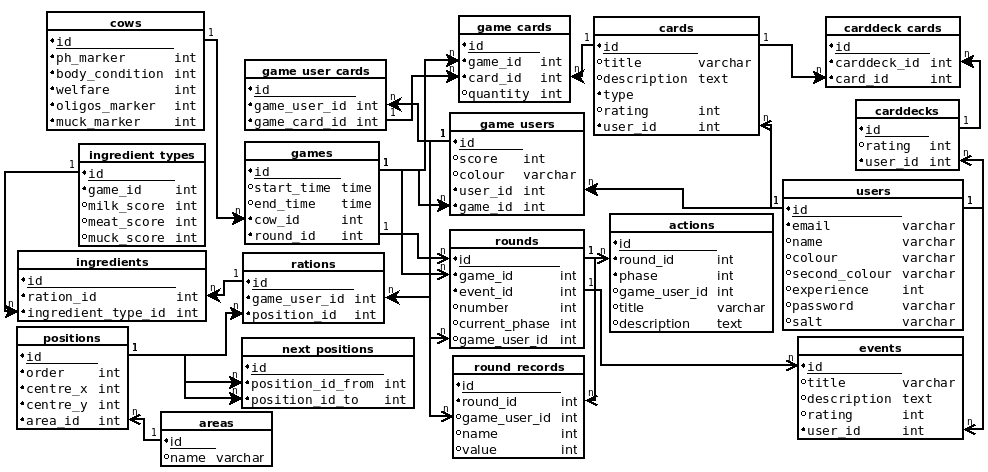
\includegraphics[width=\textwidth]{Images/app3/full-database}

\subsubsection{Conventions}
This design matches the Ruby On Rails Active Record convention. Tables names are plurals of the objects they contain. Primary keys are simply named 'id', and foreign keys are singular items \cite{ActiveRecordConvention}.

\subsubsection{Tables}
\paragraph{users} The \textbf{users} table stores details of players which allow them to login and store a few personal details. Their email, password and salt are to do with validation. Once logged in, players will be referred to by their name, and sometimes game pieces will be identified by a colour. The second colour is used in case two players in the same game have the same colour. A \textbf{users} experience will increase the more games they play.

\paragraph{game\_users} This is a table to join games with players in a many-to-many relationship. So it can be thought of as details that refer to a player and are specific to a game. A score and the determined colour (out of two possible) are needed per game the player is involved in.

\paragraph{games} One record is kept in this table for each \textbf{game} that is played. A start time and end time is recorded, and a reference to information in the \textbf{cow} table and the current round.

\paragraph{cow} The \textbf{cows} table shares a one-to-one relationship with the \textbf{games} table, only one cow is needed per game. Here values are recorded to persist the current value of markers which tell players what the state of health of the cow is in their game.

\paragraph{rounds} Rounds must be recorded, as when the game is created, the number of rounds is determined, and an event chosen for each round. So rounds identify themselves to a game, they have a number which indicates the order they appear in. The current phase is a number from one to four, relating to the possible phases. The active player is also recorded, if applicable. When the round is in the last phase, no player is active. Rounds have an event assigned when they are created, at the start of a game.

\paragraph{actions} These are created as the game progresses. They provide a record of what has happened in a round, used in the final review phase. The round and phase is necessary in an action, where as an action may be performed by a player, or may not. An example of an action is title: 'Made a ration', game\_user: 'player1', and description: 'Spent a water and energy to make a ration'. They are designed to be human readable, rather than machine readable.

\paragraph{round\_records} This table exists in order to record values, such as player's scores, from round to round. The 'name' field can be 'score' or 'cards', and the value indicates the number. This table is used for review and game statistics only.

\paragraph{rations} Each \textbf{game\_user} can have up to four rations. These are capsules for ingredients that have a set position, which can be updated by the owner in the movement phase.

\paragraph{positions} This table is necessary in order to tie the rations to the abstract shape of the game board. Positions are pre-set, and a single list is used for all games. Each position has an x and y position, which identifies where it will appear on the game board. It also has three images to represent it's shape. These are so that the area on the board can light up different colours depending if a player can move their ration to the position or not. Finally positions have an area and an order. This is so that the leading or rear ration can be determined. The leading ration is the one with the greatest area, and then the greatest order within that area.

\paragraph{next\_positions} This table defines a graph of positions. Positions can be considered nodes, and the next\_position records can be considered to be one-directional connections. So having a position it is possible to look up all the positions that lead to it, and all the positions that lead from it. This will confine where a user is allowed to move their rations. In the rumen, bi-directional connections are allowed, so two records will be needed to join neighbours.

\paragraph{areas} These correspond to the areas of the board: trough, oesophagus, rumen and intestines. They help order positions.

\paragraph{ingredients and ingredient\_types} A ration can have up to four ingredients. They are created by using cards with the corresponding ingredient, however, an ingredient record is only created when a ration is. Ingredient types store data about the number of points scored for each ingredient, as these are subject to change.

\paragraph{cards} These are all possible cards, for all possible games. Each card includes a title (eg: Medicine), a description (eg: Cow welfare +1), a rating which can be given by people who finish playing a game with that card, and the creator of the card is automatically assigned.

Another diagram exists describing the possibility of cards performing automatic effects, defined by users when they are created. But that may be implemented in a later phase, and so has been left out of this diagram for simplicity.

\paragraph{card\_decks and card\_deck\_cards} These tables organise the cards into decks, creating a many-to-many relationship between the \textbf{cards} table and the \textbf{card\_decks} table. When creating a game, a user can choose an existing card deck, or create a new one. To do this they choose the cards they want to include as well as the quantity of that card. The quantity defines how likely the card is to come from the deck, if card A has a quantity of 1, and card B a quantity of 4, card B is four times as likely as card 1, as with a real deck of cards. Card decks have a rating by those who have played a game using it.

\paragraph{game\_cards} As described above, a user chooses a deck of cards when creating a game. Because a deck could be edited by it's creator, these decks are copied to several other records, which define the unchangeable cards and quantities that will be used during the game.

\paragraph{game\_user\_cards} Within a game, a player accumulates a hand of cards. This table records this information by providing a many-to-many relationship between the \textbf{game\_users} and \textbf{game\_cards} tables.

\paragraph{events} Possible events that can happen in a game are stored in this table. The event has a title, description, rating and image. All describe the event.

\paragraph{round\_events} When a game is created it's number of rounds is determined, and an event given to each round. This table joins the rounds to events.

\subsection{Extra Database Structure}
If the project reaches the final phase, it will be necessary for cards and events to be created with automatically assignable actions that get carried out during games. To make that possible, the following database structure must be added to the existing one above.

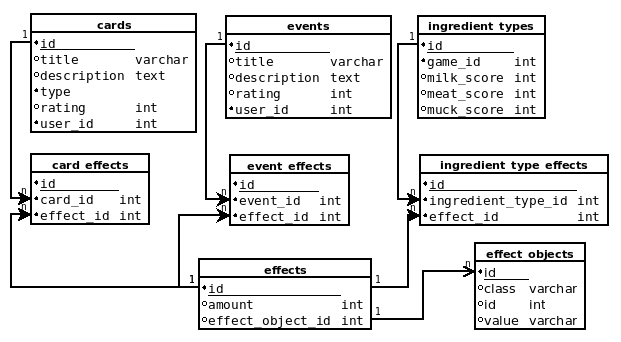
\includegraphics[width=\textwidth]{Images/app3/extra-database}

The \textbf{cards}, \textbf{events} and \textbf{ingredient\_types} tables are from the existing database. They each have a sub table which links certain instances of cards, events and ingredient types to the \textbf{effects} table. An effect is something that happens to another object in the database. The class field indicates which table that object is in, the id field picks out the row to effect, and the value says what the new, or relative value of the row should be.

An effect engine will need to be put in place to carry out these operations, but given this structure it should not be complicated to perform. If other effects are needed later, such as creating or removing an instance, they can be added as other tables that are linked to the \textbf{effects} table.

%==============================================================================
\section{RESTful API}
This section describes how the data in the previous section will be accessed via the server API. A strict standard of a RESTful API has been chosen in order to increase the organisation of interoperability between the server and client. The notation '[id]' has been used to represent a number that can be used to represent a resource.

\subsection{HTTP Operations}
Unless stated otherwise below, the HTTP operations used for URIs will follow the pattern described in this section.
\subsubsection{/resources}
This will return a collection of all the resources with the name 'resources', if the user has permission to access them. The following HTTP operations are allowed for this URI:
\begin{itemize}
	\item \textbf{POST} - creates a new 'resource'.
	\item \textbf{GET} - returns a list of all instances of 'resource'.
\end{itemize}
\subsubsection{/resources/[id]}
This will deal with a specific resource with the given id, if the user has permission to access it. The following HTTP operations are allowed for this URI:
\begin{itemize}
	\item \textbf{GET} - returns a single resource's details.
	\item \textbf{PUT} - replaces a resource's details.
	\item \textbf{PATCH} - updates part of a resource's details.
	\item \textbf{DELETE} - removes a resource.
\end{itemize}
\subsubsection{/resources/[id]/otherresources}
This will return a collection of all the resources with the name 'otherresources' that are related to the specific 'resource' identified by the id. This is only allowed if the user has permission to access them. The following HTTP operations are allowed for this URI:
\begin{itemize}
	\item \textbf{POST} - creates a new 'otherresource', but fills in the relation to the parent 'resource' automatically.
	\item \textbf{GET} - returns the 'otherresources' that are related to the 'resource', eg: are owned or created by it.
\end{itemize}
The same is true for further nested resources.
\subsubsection{/resources/[id]/otherresources/[id]}
This will deal with a specific resource with the given id, if the user has permission to access it. The following HTTP operations are allowed for this URI:
\begin{itemize}
	\item \textbf{GET} - returns a single resource's details. Resources at this level are read-only. To update or delete the resource, it can be accessed via it's base URI \textbf{/otherresources/[id]}.
\end{itemize}

\subsection{HTTP Data Types}
The API is designed to provide a service for a client. It should be possible to play a game by giving the correct values to the API without a client. However, this is not the intended use, therefore the default data type of the application will be JSON format. This is all that will be implemented for the core functionality.

When the game is fully functional, there is a chance it will be used with other clients that may demand XML or HTML data. Ruby on Rails makes it easy to return different data types, based on the requested file type. These data types can therefore be offered at a later stage.

For addressability, as far as possible resources will provide links to related resources dynamically in the data that is sent to the client.

\subsection{Resources}
\subsubsection{Users}
\begin{itemize}
	\item \textbf{/users} - a list of users.
	\item \textbf{/users/[id]} - a specific user.
	\item \textbf{/users/[id]/games} - games related to a specific user.
	\item \textbf{/users/[id]/games/[id]} - a specific game related to a specific user.
\end{itemize}
\subsubsection{Games}
\begin{itemize}
	\item \textbf{/games} - a list of games.
	\item \textbf{/games/[id]} - a specific game.
	\item \textbf{/games/[id]/cow} - a cow that is related to this game. It is a singleton.
	\item \textbf{/cows} - a list of all cow details, should you wish to know it.
	\item \textbf{/cows/[id]} - a specific cow's details, without going through the game.
	\item \textbf{/games/[id]/cards} - cards used within a game.
	\item \textbf{/games/[id]/users} - players of a game.
	\item \textbf{/games/[id]/users/[id]} - a specific player of a game.
	\item \textbf{/games/[id]/users/[id]/cards} - a list of cards belonging to a player.
	\item \textbf{/games/[id]/users/[id]/cards/[id]} - a specific card belonging to a player.
	\item \textbf{/games/[id]/users/[id]/rations} - a list of rations belonging to a player.
	\item \textbf{/games/[id]/users/[id]/rations/[id]} - a specific ration belonging to a player.
	\item \textbf{/games/[id]/users/[id]/rations/[id]/ingredients} - a list of ingredients in a specific ration belonging to a player.
	\item \textbf{/games/[id]/users/[id]/rations/[id]/ingredients/[id]} - a specific ingredient in a ration belonging to a player.
	\item \textbf{/games/[id]/round} - the current round in a game.
	\item \textbf{/games/[id]/rounds} - the current and previous rounds in a game, unless the user has permission to see all the rounds in a game.
	\item \textbf{/games/[id]/rounds/[id]} - a specific round in a game.
	\item \textbf{/games/[id]/rounds/[id]/actions} - a list of the actions that have happened in a round.
	\item \textbf{/games/[id]/rounds/[id]/actions/[id]} - a specific action within a round in a game.
	\item \textbf{/games/[id]/rounds/[id]/event} - the event that happened in a round. It is a singleton.
\end{itemize}

\subsubsection{Cards}
\begin{itemize}
	\item \textbf{/cards} - a list of all cards.
	\item \textbf{/cards/[id]} - a specific card.
	\item \textbf{/users/[id]/cards} - a list of cards the player has created.
	\item \textbf{/users/[id]/cards[id]} - a specific card that a player has created.
	\item \textbf{/decks} - a list of all decks.
	\item \textbf{/decks/[id]} - a specific deck of cards.
	\item \textbf{/decks/[id]/cards} - a list of all cards in a deck.
	\item \textbf{/decks/[id]/cards/[id]} - a specific card in a deck.
	\item \textbf{/users/[id]/decks} - a list of decks the player has created.
	\item \textbf{/users/[id]/decks[id]} - a specific deck that a player has created.
\end{itemize}

\subsubsection{Rounds and Events}
\begin{itemize}
	\item \textbf{/rounds} - a list of all the rounds. Rounds are not created by the client, so are read only.
	\item \textbf{/rounds/[id]} - a specific round.
	\item \textbf{/actions} - a list of all the actions.
	\item \textbf{/action/[id]} - a specific action.
	\item \textbf{/rounds/[id]/actions} - a list of actions that happened within a round.
	\item \textbf{/events} - a list of events.
	\item \textbf{/events/[id]} - a specific event.
	\item \textbf{/rounds/[id]/event} - the event that happened in a round. It is a singleton, and is read only.
	\item \textbf{/users/[id]/events} - a list of events created by this user.
	\item \textbf{/users/[id]/events/[id]} - a specific event created by this user.
\end{itemize}

\subsubsection{Positions and Areas}
Positions and areas are read only. They are the same for all games. Rations are updated with positions.
\begin{itemize}
	\item \textbf{/positions} - returns a list of all positions, in order.
	\item \textbf{/positions/[id]} - a single position's details.
	\item \textbf{/positions/[id]/next}  - a list of all positions from this position.
	\item \textbf{/positions/[id]/previous} - a list of all positions going to this position.
	\item \textbf{/areas} - a list of all areas, in order.
	\item \textbf{/areas/[id]} - a single area's details.
	\item \textbf{/areas/[id]/positions} - a list of positions in this area, in order.
	\item \textbf{/positions/[id]/graph/[number]} - uses the positions like a graph. A number must be supplied. The result will be a recursive list of positions, each with an array of their next positions. The depth is the number supplied.
\end{itemize}

%==============================================================================
\section{Client Structure}

\subsection{Pages}
\includegraphics[width=\textwidth]{Images/app3/pages}
This diagram shows the pages needed for the application. Four phases are shown, indicating which pages are required for which phases of development outlined in the requirements analysis. The following description focuses on the first phase, the pages necessary for creating a working application.

\subsubsection{Index Page}
\begin{center}
	\fbox{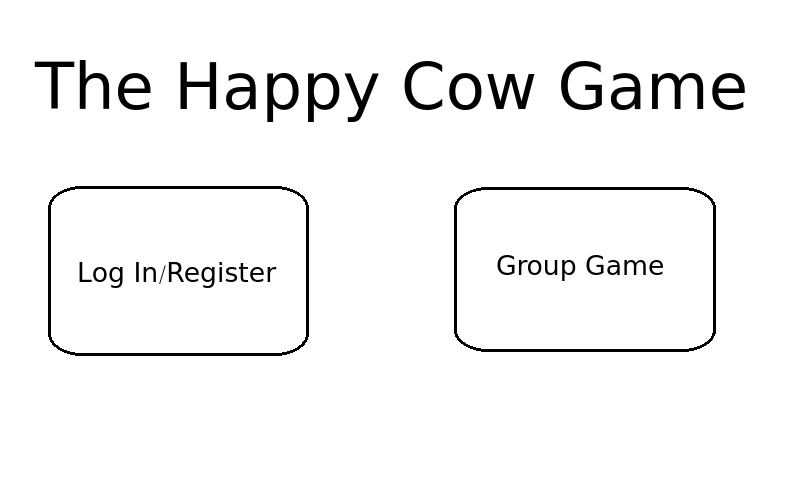
\includegraphics[width=4in]{Images/app3/pages-1-index}}
\end{center}
This is the index page, the first page a user sees. It gives the options of loging in and registering, or creating a group game. A group game will only be possible in a later phase of development.

\subsubsection{Login Page}
\begin{center}
	\fbox{\includegraphics[width=4in]{Images/app3/pages-2-login}}
\end{center}
The login page allows a user to authenticate themselves with their email and password. There is also an option to register, if the user is new to the site.

\subsubsection{Register Page}
\begin{center}
	\fbox{\includegraphics[width=4in]{Images/app3/pages-3-register}}
\end{center}
The register page is designed to look similar to the login page, but with a few more feilds. This means that when choosing to register instead of logging in, the page updates and simply asks for a name and confirmation of the password as well.

\subsubsection{Games List Page}
\begin{center}
	\fbox{\includegraphics[width=4in]{Images/app3/pages-4-games}}
\end{center}
The game list page is the entry point for games, and other options available to a user. From here a user can see different games they are involved in, and a few details of each. Options allow a user to resume a game, or leave it if they don't want to play anymore. Other menu buttons allow a user to begin a game and view their profile.

\subsubsection{Profile Page}
\begin{center}
	\fbox{\includegraphics[width=4in]{Images/app3/pages-5-profile}}
\end{center}
This page allows a user to view and edit their personal details. The details needed to register are on the right. When updating a password or email, a confirmation email will be sent. The details on the right are to do with how users are represented in a game.

\subsubsection{Game Setup Page}
\begin{center}
	\fbox{\includegraphics[width=4in]{Images/app3/pages-6-new}}
\end{center}
This page allows a user to create a new game. They can choose a name, a deck of cards to use, and the length of the game. They can also send invites to other players. At first these will be a link allowing a player to join a game themselves, but later if time allows, will be a message within the game.

For players who aren't creators but are joining a game, the edit buttons will not be available. The only action possible will be 'Join' or 'Leave'.

\subsubsection{Play Game Page}
This page is far more detailed than those above, and is described in the following section. When players resume a game, this page is loaded and guides them through the various changes and phases of a game.


\subsection{Game Play User Interface}
The game play page is a single page application. That means it does not require a page load to update data on the page. Instead this is done behind the scenes via Ajax requests to the server. The methods to do this are discussed in the next section. Here the layout of this SPA is considered.

\subsubsection{Menu}
Basic controls of the game appear in a menu at the top of the screen. These include:
\begin{itemize}
	\item A \textbf{Main Menu} with options to return to the game list page, or log out. More features can be added to this list if time allows, such as view statistics of the game.
	\item An overview of the \textbf{Score}. This shows the authenticated player's score, and when clicked, ranks the players in order of score.
	\item \textbf{Messages} will not be implemented in the core functionality.
	\item The \textbf{Round} button shows the current round, and also allows players to see the review phases of previous rounds.
	\item The \textbf{Phases} buttons show the current phase, but give players the ability to visit previous phases. The current phase may have a series of actions. Yet if the current phase is the cards phase, a player can still see the state of the board in the movement phase, but cannot perform any actions.
	\item The \textbf{Active Player} button shows the player whose turn it currently is. A drop down also shows the current order of play, as this changes from round to round.
\end{itemize}
\begin{center}
	\includegraphics[width=5in]{Images/app3/ui-menu}
\end{center}

\subsubsection{Cow Information}
This section of the user interface, like the menu, is always visible. It shows the state of the cow.
\begin{center}
	\includegraphics[width=2.5in]{Images/app3/ui-cow-info}
\end{center}

Five markers are shown: Welfare, Body Condition, Rumen PH, Muck and Oligos. These are updated as the game progresses and give an overview of various statistics.

The points that ingredients score are also shown, as these can change. This gives players an idea of what ingredients to include in their rations, and where to try and get their rations absorbed.

Finally there are a few events that remain from turn to turn. These are shown at the bottom and updated as events change.

\subsubsection{Event Phase}
The first of the four phases is the Event Phase. An event will usually have consequences for a player, but these happen later in the game play. The only action available to a player is to review the phase and move on to the cards phase. An example event is shown below.
\begin{center}
	\includegraphics[width=\textwidth]{Images/app3/ui-phase-event}
\end{center}

\subsubsection{Cards Phase}
The second phase is the cards phase. Players receive two new cards at the start of this phase, and can see their deck in a scrollable list of cards. Actions are shown below the cards, and for more details a player can click on a card.

Below the list of cards a player can view their existing rations, and create a new ration if they have at least one ingredient and do not already have four rations. By clicking the 'Use' button below an ingredient, the ingredient appears in the list of ingredients ready to be made into a ration. When ready the player can click to create the ration.
\begin{center}
	\includegraphics[width=\textwidth]{Images/app3/ui-phase-cards}
\end{center}

Only one ration can be made per player, per round. A modal is displayed to confirm that the user wants to create a ration with the selected ingredients. If they are sure, they confirm their choice and the corresponding ingredient cards in their hand are removed.
\begin{center}
	\includegraphics[width=\textwidth]{Images/app3/ui-phase-cards-create}
\end{center}

The player can continue to perform actions on action cards, or discard cards. When they are ready to move on, they end the phase.

\subsubsection{Movement Phase}
The third phase is the movement phase. In this phase the player must select a ration to move, and then select a movement amount offered by the dice. So there are 3 actions within this phase:
\begin{itemize}
	\item Select a ration. The player can click on the rations in the bottom control bar, and the board will move so that the ration is shown in the centre. They then confirm their choice of ration to move.
	\item Select a movement amount. Only once a ration is selected are the movement amounts for that ration calculated and shown. The player can then select the different dice, and the squares where the ration can move are highlighted.
	\item Move the ration. By clicking on one of the highlighted squares, the player confirms their choice of movement. As a player clicks on a square, the ration is shown to 'hop' to that square. The player must keep clicking until all the movements are used up.
\end{itemize}
Once all the movements are used up for the selected ration, the player's movement phase is automatically over.
\begin{center}
	\includegraphics[width=\textwidth]{Images/app3/ui-phase-move}
\end{center}

\subsubsection{Review Phase}
The fourth and final phase is the review phase. No actions are available, but to confirm that they are ready to move on. The player is shown a list of actions that have happened this round, and the current level of points for the round.
\begin{center}
	\includegraphics[width=\textwidth]{Images/app3/ui-phase-review}
\end{center}

When all the players indicate they are ready to move on, the next round begins.

\subsection{AngularJS}
This section delves into the different components that make up the game play page. AngularJS uses controllers and services to separate concerns. Controllers perform logic on data that is represented in the Document Object Model (DOM), and therefore each 'functional area' of a page (called the 'view' in Angular terms), should be operated by a separate controller \cite{AngularBook}, page 28. Services, on the other hand, can be created when needed to perform actions within the controllers. Examples are routing and data storage.

\subsubsection{Controllers}
The controllers needed to display and update data within the game play page are listed below.
\begin{enumerate}
	\item \textbf{MenuController} This is a parent controller for the operations of the menu bar at the top of the page.
	\begin{enumerate}
		\item \textbf{MenuViewController} This controller manages a drop down menu with options to leave the game play area, logout, ect.
		\item \textbf{ScoreViewController} This controller manages a drop down menu showing the players in order of score. It also displays the score and position of the player. Further information about scores throughout the game, and how to score points, can be accessed.
		\item \textbf{RoundViewController} This controller manages a drop down menu showing the number of rounds played, and the current round. It offers the option to review previous rounds, allowing users to access the review information from previous rounds.
		\item \textbf{PhaseViewController} This controller shows the current phase by highlighting the current phase and updating the phase on user clicks.
		\item \textbf{Player View Controller} This controller shows the active player, and manages a drop down menu showing the player playing order.
	\end{enumerate}

	\item \textbf{CowController}
This is a parent controller for the cow information display, to the right of the page.
	\begin{enumerate}
		\item \textbf{CowStatsController} This controller manages the progress bars which show the welfare, body condition, rumen PH, muck and oligos markers. These need to be updated automatically as the game progresses.
		\item \textbf{IngredientValueController} This controller manages the table of ingredient values, updating their values as events cause changes.
		\item \textbf{CowEventsController} This controller manages the Pregnancy, Diseases and Weather areas that show changes to cow behaviour caused by events.
	\end{enumerate}

	\item \textbf{PhaseController}
This is a parent controller for the display of the main area of the board. It is changed as players view different phases using the PhaseViewController.
	\begin{enumerate}
		\item \textbf{EventController} This controller manages the template showing the event of the round.
		\item \textbf{CardsController} This controller is a parent of those which manage the actions related to cards.
		\begin{enumerate}
			\item \textbf{CardDeckController} This controller manages actions of cards, and also displays modals with more details of the cards and their causes.
			\item \textbf{CreateRationController} This controller manages uses of ingredients and displays rations as they are created. A modal is provided to review a ration to confirm creation.
			\item \textbf{ExistingRationsController} This controller shows the existing rations, and manages pop-ups showing their position. If a ration is created, it updates to show it.
		\end{enumerate}
		\item \textbf{MovementController} This controller is a parent of those which control movement of rations.
		\begin{enumerate}
			\item \textbf{BoardController} This controller manages the zooming, scrolling, and automatic changes of the board as rations are selected.
			\item \textbf{RationMovementController} Once a ration is selected, this controller manages the actions needed to highlight it, show it's possible movements and update it's position.
			\item \textbf{RationSelectionController} This controller manages the selection of controllers and dice to decide it's movement. Rations and dice need to be disabled once one is chosen.
		\end{enumerate}
		\item \textbf{ReviewController} This controller manages the template showing the actions that have happened during the round.
	\end{enumerate}
	\item \textbf{AlertsController} This controller manages the alerts created by user actions, displaying and deleting them.
\end{enumerate}

\subsubsection{Services}
Currently known services needed are:
\begin{itemize}
	\item An \textbf{\$resource} service. This extends the \$http service and is especially designed for use with a RESTful API. It will perform requests to the server. Many of the controllers will need to do this to perform actions players have requested, and update the page with the responses.
	\item An \textbf{\$animate} service. This helps angular perform basic animations on elements within the page.
	\item An \textbf{Alerts} service. This will allow any controller to create alerts. The AlertsController will be integrated to display alerts that are generated by this service.
	\item A \textbf{LocalStorageModule} service (\url{https://github.com/grevory/angular-local-storage}). This will be used during development to store data instead of sending it to the server. Once the prototype is complete, this will be replaced by the \textbf{\$http} service.
\end{itemize}

%==============================================================================
\section{Detailed Design Sections}
Some areas of the game will be straight forward, and simply involve implementing the API and client side structure above. Other sections require some more thought, however. The aim of this section is to identify and briefly consider these sections.

\subsection{Drawing and Moving Rations}
Once created, a ration has a place on the game board. This has to be both persisted in a database, and represented to the user. To do this, a table of positions is stored, the same list exists for every game instance. Positions need to know where they should appear on the game board. For this reason they have a centre position, indicated by an x and y value. These values correspond to a position on the game board, measured from the top left.

A ration has a record of it's position. It always has a position. If it is absorbed or leaves the cow, it scores points and is then removed. A ration can therefore, use it's position's coordinates to decide where it appears on the board.

\begin{center}
	\fbox{\includegraphics[width=5in]{Images/app3/detail-1}}
\end{center}

As well as x and y coordinates, positions also have a concept of 'next positions'. This means that a position knows which positions a ration can move to from it, and vice versa. This creates a data structure called a graph, where nodes (positions) are connected by one-way relations. When moving a ration, it is therefore possible to look up which positions can be moved to from the current position. This is possible using the server API \textbf{/positions/[id]/graph/[number]} where [id] is the current position, and [number] is the value of the dice.

\begin{center}
	\fbox{\includegraphics[width=5in]{Images/app3/detail-2}}
\end{center}

In this example, the ration can move 2 spaces. Because the ration is on a bend, the only relations between positions are forwards, down the oesophagus. The ration must move through the first position, so it is marked in orange, but can only finish in the second position, so it is marked in green. These colours help players to see where their rations are allowed to go as they select different dice, and think about which movement to use.

The final challenge is animating the movement. A ration moves one position at a time, as the player must choose which position to move to if there is more than one option. The animation can be done using the coordinates of the two positions, the current position of the ration and the new position of the ration. The difference of the coordinates for x and y is determined, and then divided by 10. The ration is then moved by this amount every 50 mili-seconds. After half a second the animation will be complete.

\subsection{Ordering Positions}
To be able to order rations based on their progress through the cow digestive system, positions need an order. When rations are displayed in the cards or movement phase, they can then be ordered by the order of their positions, without having to work out an order using the graph of positions, which would be computationally expensive. In the oesophagus and intestines the order is fairly straight forward, and can be determined based on the distance from the entry point. In the rumen, the order will be across, so the numbers increase as they go down and to the right.

\begin{center}
	\fbox{\includegraphics[width=4in]{Images/app3/detail-3}}
\end{center}

As well as providing an order of rations that can be used for display, and resolving some actions, an order to positions as an added advantage when it comes to pushing rations. Rations can be pushed by other rations with more fiber. To work out the direction the attacked ration should be pushed in, the order of positions can be used. If the order of the position the pushing ration came in is less than the order of the current position, then the attacked ration must be pushed to a position with a larger order.

\begin{center}
	\fbox{\includegraphics[width=4in]{Images/app3/detail-4}}
\end{center}

In the example above a ration in position ordered 8 is moving to position ordered 12 and has fiber, so can push a ration already on that position. But which direction should the ration be pushed? It is obvious to us, but not with a graph data structure. Instead of comparing coordinates, which could become very complicated in the oesophagus or intestines, the order can be used. There are four possible positions: 7, 8, 17 and 18. The pushing ration is from the second lowest position, so it pushes to the second highest position. If it came from the lowest position it would push to the highest position, and vice versa.

\subsection{Invites}
When a player creates a game, he will want other players to join in. This is done through invitations. One player has control over the creation of a game in order to avoid conflicts when setting a game up.

Initially, to invite another player to a game, the creator of the game will have to send an invitation as a URL to a page via some form of social media. That will allow the player they contact to login, and visit the same game creation page. The player joining will see the name and choice of cards for the game, as well as the list of players who have already joined the game, but they will only be able to perform two actions: join or leave. If they join, a \textbf{game\_users} record is created for that player. If they then decide to leave the game, that record is deleted.

Messages are an extra feature of the project, to be implemented in a later phase. An invitation will be a special form of message that appears in a list of invites for each user. It is essentially an in-game message of the type above that directs a player to the game setup page. They then join or leave as described above.

\chapter{Test Results}
This section contains the test results for server side automated tests and application usability tests. All automated tests listed here passed.

\section{Automated Tests}
  \subsection{Unit Tests}
The unit tests are located in \textit{/app/test/models}. Each test described below will have at least one assertion that passes, but many have two or more.
\subsubsection{Action Model Tests}
\begin{itemize}
	\item test that a game has several actions
	\item test that playing a card creates an action
	\item test that creating a ration creates an action
\end{itemize}

\subsubsection{Card Model Tests}
\begin{itemize}
	\item test that a card has a creator
\end{itemize}

\subsubsection{Carddeck Model Tests}
\begin{itemize}
	\item test that a card deck has a creator
	\item test that a card deck has a number of cards
\end{itemize}

\subsubsection{Cow Model Tests}
\begin{itemize}
	\item test that a cow belongs to a game
	\item test increasing the cow's pH marker within it's range
	\item test increasing the cow's pH marker beyond it's range
	\item test decreasing the cow's pH marker within it's range
	\item test decreasing the cow's pH marker below it's range
	\item test that an more energy than water in the cow's rumen decreases the rumen pH level
	\item test increasing the cow's welfare marker to 1
	\item test increasing the cow's welfare beyond it's range
	\item test decreasing the cow's welfare to -1
	\item test that decreasing the cow's welfare to -7 will kill the cow and end the game
	\item test increasing the cow's body condition to 1
	\item test increasing the cow's body condition beyond it's range
	\item test decreasing the cow's body condition to -1
	\item test that decreasing the cow's body condition to -3 will kill the cow and end the game
	\item test that setting a weather event resets the cow's weather event
	\item test that setting a disease event resets the cow's disease event
	\item test that setting the pregnant event resets the cow's pregnancy event
	\item test that the cow's scores for oligos is 10 by default
	\item test that when the cow's oligos marker is at 1, it's oligos score is 2
	\item test that when the cow's oligos marker is at 2, it's oligos score is 0 and welfare decreases
	\item test that resetting the cow's oligos marker puts it's oligos score back at 10
	\item test that when increasing the cow's muck marker to 3 welfare decreases 1
	\item test that when increasing the cow's muck marker to 5 welfare decreases 2
	\item test that when increasing the cow's muck marker to 6 welfare decreases 3
	\item test that when increasing the cow's muck marker to 7 welfare decreases 4
	\item test that killing the cow sets the game to a failed stage
	\item test that the method to check if the cow is constipated works
	\item test that the method to check if the cow has mad cow disease works
	\item test that the method to check if the cow has diarrhea works
	\item test that the method to check if the cow is in hot weather works
	\item test that the method to check if the cow is in cold weather works
\end{itemize}

\subsubsection{Event Model Tests}
\begin{itemize}
	\item test making the constipation event the active disease event
	\item test making the diarrhea event the active disease event
	\item test making the cold weather event the active weather event
	\item test making the hot weather event the active weather event
	\item test making the good weather event the active weather event
	\item test making the mad cow crisis event the active disease event
	\item test making the mad cow crisis event inactive again
\end{itemize}

\subsubsection{Game Model Tests}
\begin{itemize}
	\item test beginning a game without any users
	\item test beginning a game with a higher minimum number of rounds than maximum
	\item test beginning a game already in the playing phase
	\item test that beginning a game moves it's stage to 1
	\item test that beginning a game populates the game cards from the card deck
	\item test beginning a game creates a cow, motile pieces and ingredient types
	\item test that beginning a game makes the correct number of rounds
	\item test that in a new game, the last event is the slaughter house
	\item test that in a new game every player has 2 cards
	\item test that the game's function to get the next player works
	\item test that a ration absorbed as milk gives a score of 2
	\item test that the absorbed function only works if the ration is in a viable position
	\item test that a ration absorbed as milk, when the cow is pregnant, gives a meat score of 2
	\item test that a ration absorbed as meat gives a score of 2
	\item test that a ration absorbed as muck gives a score of 2
	\item test that a ration with two oligos scores 10 for the first and 2 for the second
	\item test that a ration absorbed when the cow is cold gets 1 less point per ingredient
	\item test that rations in the trough automatically shuffle down
	\item test that a game user is created by copying in user details
	\item test that a game user cannot be created once the game is begun
	\item test that a user cannot be created twice as a game user in a game
	\item test that the assign cards function gives a number game cards to the specified game user
	\item test that the winner of the game gets 3 experience and everyone else gets 1 if the welfare is 2
	\item test that in the case of a tie, neither player gets more experience
	\item test that when the cow dies players lose a lot of experience
	\item test that the card balance function distributes more ingredients at the beginning, and more actions at the end
	\item test that you cannot create a game user without a user
\end{itemize}

\subsubsection{GameUserCard Model Tests}
\begin{itemize}
	\item test that you cannot use a card with no specified action
	\item test that you cannot use a card that is not an action card
	\item test the action of the card acidodis plus
	\item test the action of the card acidodis minus
	\item test the action of the card rumination
	\item test the action of the card thief
	\item test the action of the card vet
	\item test the action of the card clean stables
	\item test the action of the card animal welfare activists
	\item test the action of the card deficiency
	\item test the action of the card medical insurance
	\item test the action of the card saponins (fiber in rumen turned to protien)
	\item test the action of the card probiotics
	\item test the action of the card farm improvements
	\item test the action of the card bioreactor
	\item test the action of the card high sugar grass
\end{itemize}

\subsubsection{GameUser Model Tests}
\begin{itemize}
	\item test that a game user belongs to a game
	\item test that a game user belongs to a user
	\item test that a ration will not be created without ingredients
	\item test that a ration will not be created with ingredients that do not belong to the new owner
	\item test that a ration will be created with correct ingredients
	\item test that a user's cards used to create a ration are destroyed
\end{itemize}

\subsubsection{IngredientCat Model Tests}
\begin{itemize}
	\item test that an ingredient category has many ingredients
	\item test that an ingredient category has a game
	\item test that the method to get ingredient category scores works for water
	\item test that the method to get ingredient category scores works for energy
	\item test that the method to get ingredient category scores works for protein
	\item test that the method to get ingredient category scores works for fiber
	\item test that the method to get ingredient category scores works for olgios
	\item test that the oglios score decreases when oligos is absorbed
\end{itemize}

\subsubsection{Ingredient Model Tests}
\begin{itemize}
	\item test that an ingredient has a ration
	\item test that an ingredient has an ingredient category
\end{itemize}

\subsubsection{Motile Model Tests}
\begin{itemize}
	\item test that a motile element has a game
	\item test that a motile element has a position
	\item test the result of moving a motile element to an empty place
	\item test that a motile element cannot not move to the exit of the rumen
	\item test the result of moving a motile element onto a ration
\end{itemize}

\subsubsection{Move Model Tests}
\begin{itemize}
	\item test setting the dice for a move
	\item test setting the dice for a move with water
	\item test setting the dice for a move with a low rumen pH
	\item test setting the dice for a move with a high rumen pH
	\item test setting the dice for a move with the cow constipated
	\item test setting the dice for a move with the cow having diarrhea
	\item test that with a selected dice, a ration can move between positions
	\item test that a ration is consumed when ending it's turn on the milk position
\end{itemize}

\subsubsection{Position Model Tests}
\begin{itemize}
	\item test that a ration cannot move to a position with a motile element
	\item test that a position with no ration or motile element is free
	\item test that a ration with 1 fiber cannot move to a position occupied by a ration with 2 fiber
	\item test that a ration with 2 fiber can move to a position occupied by a ration with 1 fiber
\end{itemize}

\subsubsection{Ration Model Tests}
\begin{itemize}
	\item test that the method describe\_ingredients returns a string with labels of the ration's ingredients
	\item test that the method has\_type correctly determines if a ration has an ingredient
	\item test that the method count\_type correctly returns the number of ingredients a ration has of that type
\end{itemize}
	
  \subsection{Functional Tests}
The functional tests are located in \textit{/app/test/controllers}. Each test described below will have at least one assertion that passes, but many have two or more.
\subsubsection{Actions Controller Tests}
\begin{itemize}
	\item test the request should not get the index method, without authentication
	\item test the request should not get a specific record, without authentication
	\item test the request should get the index method
	\item test the request should get the show method for an authenticated user
\end{itemize}

\subsubsection{Carddecks Controller Tests}
\begin{itemize}
	\item test the request should not get the index method, without authentication
	\item test the request should not get a specific record, without authentication
	\item test the request should get the index method
	\item test the request should get the show method for an authenticated user
\end{itemize}

\subsubsection{Cards Controller Tests}
\begin{itemize}
	\item test the request should not get the index method, without authentication
	\item test the request should not get a specific record, without authentication
	\item test the request should get game cards filtered by games
	\item test the request should get game user cards filtered by game users
	\item test the request should not get game user cards filtered by game users, with an unauthenticated game user
	\item test the request should get  a card for an authenticated user
	\item test the request should get a game card filtered by a game
	\item test the request should get a game user card filtered by a game user
	\item test the request should not get a game user card filtered by a game user, with an unauthenticated game user
	\item test the request should not get a game card filtered by a game, with a non playing user
	\item test the request should update a record of a card
	\item test the request should update a record of a game card
	\item test the request should not update a record of a game user card for an unauthenticated user
	\item test the request should update a record of a game user card for an authenticated user
	\item test the request should not use an ingredient card
	\item test the request should not update a game user card without a use parameter
	\item test the request should not delete a card
	\item test the request should not delete a game card
	\item test the request should delete a game user card for an authenticated user
\end{itemize}

\subsubsection{Events Controller Tests}
\begin{itemize}
	\item test the request should not get the index method, without authentication
	\item test the request should not get a specific record, without authentication
	\item test the request should get the index method
	\item test the request should get the show method for an authenticated user
\end{itemize}

\subsubsection{GameUser Controller Tests}
\begin{itemize}
	\item test the request should not get the index method, without authentication
	\item test the request should not get a specific record, without authentication
	\item test the request should not update a record, without authentication
	\item test the request should get the index method
	\item test the request should get the show method for specific user only
	\item test the request should update a record for an authorised user
	\item test the request should delete a record for a specific user only
	\item test the request to delete a game user should destroy a game because they are the only game user
\end{itemize}

\subsubsection{Games Controller Tests}
\begin{itemize}
	\item test the request should not get the index method, without authentication
	\item test the request should not get a specific record, without authentication
	\item test the request should get the show method
	\item test the request should not get the show method for a user who is not part of the game
	\item test the request should allow finishing a turn for the current player
	\item test the request should not allow finishing a turn for a player other than the current player
	\item test the request should not allow finishing a turn for user who is not a player
	\item test the request should not allow an update of game details once the game is in stage two
	\item test the request should allow an update of game details for a game in stage one
	\item test the request should not allow an update of game details for a non creator
	\item test the request should not allow a non-creator to begin a game
	\item test the request should allow the game creator to begin a game
\end{itemize}

\subsubsection{Moves Controller Tests}
\begin{itemize}
	\item test the request should not get the index method, without authentication
	\item test the request should not get a specific record, without authentication
	\item test the request should filter the index method when nested under rounds
	\item test the request should filter the index method when nested under game users
	\item test the request should not filter the index method when nested under game users, with an unauthenticated game user
	\item test the request should get the show method for an authenticated user
	\item test the request should not get the show method when filtered by a game user, with an unauthenticated game user
	\item test the request should not get the show method when filtered by a round, with playing user who is not in the round
	\item test the request should not update a record for an unauthenticated user
	\item test the request should not update a record for an authenticated user who does not supply an update action
	\item test the request should update a record when confirming a ration for an authenticated user
	\item test the request should not update a record when confirming a ration when it is already confirmed
	\item test the request should not update a record when confirming a ration when the ration does not belong to the authenticated user
	\item test the request should not update a record when making a move when no ration is confirmed
	\item test the request should update a record when making a move when a ration is confirmed
	\item test the request should not update a record when making a move to change the selected die
	\item test the request should not update a record when making a move to move to a ration to a non-neighbouring position
	\item test the request should not update a record when making a move to move a ration too far
\end{itemize}

\subsubsection{Positions Controller Tests}
\begin{itemize}
	\item test the request should not get the index method, without authentication
	\item test the request should not get a specific record, without authentication
\end{itemize}

\subsubsection{Rations Controller Tests}
\begin{itemize}
	\item test the request should not get the index method, without authentication
	\item test the request should not get a specific record, without authentication
	\item test the request should get the index method
	\item test the request should get the index method when filtered by the game user
	\item test the request should get show method for an authenticated user
	\item test the request should create a ration for an authenticated user
	\item test the request should not create more than one ration a turn
	\item test the request should not create a ration using an un-owned ingredient
	\item test the request should not create a ration with non-ingredient cards
	\item test the request should not create a ration for an unauthorised user
\end{itemize}

\subsubsection{Rounds Controller Tests}
\begin{itemize}
	\item test the request should not get the index method, without authentication
	\item test the request should not get a specific record, without authentication
	\item test the request should get the index method
	\item test the request should get the show method
\end{itemize}

\subsubsection{Users Controller Tests}
\begin{itemize}
	\item test the request should not get the index method, without authentication
	\item test the request should not get a specific record, without authentication
	\item test the request should not update, without user authentication
	\item test the request should get the index method
	\item test the request should get the show method for a specific user only
	\item test the request should update a record for a specific user only
	\item test the request should update a record with a user's users name, email, colour and password
	\item test the request should not login a user with an incorrect username
	\item test the request should not login a user with an incorrect password
	\item test the request should login a user with with a correct username and password
	\item test the request should not create a user with an existing username
	\item test the request should not create a user without a password
	\item test the request should create a user given a username, name and password
\end{itemize}

\section{Usability Tests}
	Testing was done over the period of two months. Testers were invited to play the game, usually with little instruction, but help as they went along if they became confused. This helped ascertain how difficult the learning curve of using the application was. Feedback from users is shown below.

\subsection{Feedback from the 12th of March}
\begin{itemize}
	\item It is not clear to know how to get started when playing a game. - Developer's Note: some improvements have been made to usability, but it is still an ongoing issue to consider.
	\item No obvious instructions, rules or tutorial (or at least I did not find them). - Developer's Note:  these have now been added, but could be improved.
	\item Log out button does not work, and drop down menu stays after returning to main page. Developer's Note: the log out button and drop down have been fixed.
	\item I cannot actually change card deck when creating a game. - Developer's Note: there is currently only one card deck to choose from, adding more is an enhancment. Perhaps they should be removed until then to avoid confusion.
	\item The zoom and arrow keys in 'movement' do not work as expected. - Developer's Note: the zoom did not work correctly and was consequently removed, the arrow keys to move around the board were fixed.
	\item I cannot work out how to do anything in any of the turn phases. - Developer's Note: effort has been made to make this clearer by listing instructions one at a time.
	\item I played several rounds until the game ended, but was not able to do anything. - Developer's Note: it needs to be clearer what the user is meant to do in a game.
\end{itemize}

\subsection{Feedback from the 26th of March}
\begin{itemize}
	\item Spelling error on user profile page, 'confrim password' is spelled incorrectly. - Developer's Note: this has been fixed.
	\item Spelling error across the application, 'PH' needs to be written as 'pH' - Developer's Note: this has been fixed in some places.
	\item Ingredient instructions are not clear enough, and misleading. They need to be improved. - Developer's Note: changes to instructions are now complete.
	\item The layout of text in the review phase is hard to read, consider changing the layout. - Developer's Note: the layout has been fixed.
	\item The phase screen should move to the next phase automatically when the turn is updated - Developer's Note: automatic moving of the phase screen is complete.
	\item The drop down allowing review of previous rounds does not update automatically - Developer's Note: this has been fixed.
	\item The disease information in the cow information does not update automatically. - Developer's Note: this is fixed but for instance of first event.
	\item The phase controls are not obvious, consider a layout that does not require their existence. - Developer's Note: a new design has been formulated, but time has not allowed it to be implemented yet.
	\item Rations get 'stuck' behind others, as there is no way to finish a turn if the movement of the ration is not complete - Developer's Note: this has been fixed.
	\item Notices do not disappear automatically, particularly end of turn notices. - Developer's Note: partly fixed, notices created in batches do not automatically disappear.
	\item The text pointing to the milk square of the board should change to 'meat' when the cow is pregnant. - Developer's Note: This change has been made.
	\item The last two squares of the oesophagus are not joined. - Developer's Note: this has been fixed.
	\item Update of positions sometimes allows movement to positions that are too far away. Consider changing the way this update is performed. - Developer's Note: the update of positions has been radically changed, causing this error to be fixed.
	\item A ration should be removed if all it's ingredients are destroyed by motile elements. - Developer's Note: complete, but not thoroughly tested.
	\item A spelling error in the message about a motile collision: 'piece' is spelled incorrectly. - Developer's Note: this has been fixed.
	\item A pop-up in the cards phase should ask the user if they want to finish their turn, as the button can be mistaken for the 'create ration' button. - Developer's Note: no longer an issue with new layout of button instructions.
	\item An error occurred when ending a turn. - Developer's Note: there must have been an error. Testing has fixed many issues, and this one has not reoccurred.
	\item Text description of ingredients does not fit into the boxes when reviewing the selected ingredients for a ration. - Developer's Note: this has been fixed.
	\item Rations are not showing their owner's colour. - Developer's Note: this has been fixed.
	\item The constipation and diarrhea event cards do not correctly describe the actions of the events. - Developer's Note: the descriptions have been updated.
	\item Alerts should disappear when a player performs a new major action. - Developer's Note: this will be an enhancement.
	\item Random card generation produces too much oligos. Begin with twice as many other ingredients as olgios to randomly select from. - Developer's Note: this has been implemented.
	\item The deficiency card does not reset the oligos score. - Developer's Note: the card action is now working.
	\item A ration with more than four ingredients was created, although four were submitted. - Developer's Note: this was an error on the development version, it is not an issue on the liver server.
	\item The pregnancy event should show the beginning and completion of pregnancy, instead of being the same event for both. - Developer's Note: an enhancement.
\end{itemize}

\subsection{Feedback from the 31st of March}
\begin{itemize}
	\item Position updating still has rendering problems. Make sure that the current position of the ration is not a possible position to move to. - Developer's Note: some errors remain, but many have been fixed.
	\item Make it possible to skip the turn if no dice have a number. Low rumen pH makes this quite a reasonable occurrence. - Developer's Note: this is still an outstanding issue.
	\item The acidodis card gave a message but produced no effect. - Developer's Note: this is also an outstanding issue, despite testing which should have fixed it.
	\item A waiting notice would give helpful feedback to users when there is a long server requests. - Developer's Note: a waiting notice for creating a game has been implemented, but futher notices would be helpful.
	\item Provide an option for a faster game that has a shorter cow digestive system. - Developer's Note: this must be an enhancement, it will take a lot of work.
	\item Milk and meat squares can be hard to hit with a ration, perhaps make two of each type so that it is easier to get your ration absorbed. - Developer's Note: this will be an enhancement, it is not vital to game play.
	\item Provide visual feedback when the cow is sick, and dead. - Developer's Note: this will be an enhancement, it is not vital to game play.
\end{itemize}

\subsection{Feeback from the 2nd of April}
\begin{itemize}
	\item New players need to know strategies of the game, and how to feed the cow by creating rations. - Developer's Note: a design for an enhancement to give players hints has been created, but not implemented.
	\item An introduction to the game, not as long as the page instructions, but that can be cancelled would be helpful. - Developer's Note: this will be added at a later stage.
	\item Make it obvious that the objective of the card's phase is to create a food ration. One way to do this would be by telling a user use ingredient cards. - Developer's Note: this has been accomplished by changing the instructions.
	\item The colouring of the possible positions to move to can be confusing. Use a green square instead of a blue one. - Developer's Note: this has been implemented.
	\item Rations move over each other, they should be able to push each other, but only if they have more fibre. - Developer's Note: this has been implemented as it was part of the requirements.
	\item Put the player name before instructions or the cards, so that in crowd games you know whose turn it is easily. - Developer's Note: this has been done.
	\item Put a use button by the cards so that once you know what they do you don't have click on their details to use them. - Developer's Note: this has been done.
\end{itemize}

\subsection{Feedback from the 14th of April}
\begin{itemize}
	\item Rations and motile elements are appearing on top of other sections of the screen outside of the game board area. - Developer's Note: this is still an outstanding issue, some game board elements have been fixed, but z-index adjustment is a fiddly thing. 
	\item Some alerts, to do with ration creation, do not automatically fade away. - Developer's Note: ration creation alerts now fade, but others still remain.
	\item In a crowd game, a popup between turns to let the user know whose turn it is next could be useful. As long as there is a 'do not show again' button. - Developer's Note: this will be an enhancement, it should be tried and user feedback can decide if it remains.
	\item Allow players to move the entire ration movement in one click by clicking on the end of the route that rations can take. - Developer's Note: this has been done.
	\item Some messages should wait longer before disappearing, as they have a long message but don't give time for the user to read them. - Developer's Note: where this has been noticed as an issue it has been fixed.
	\item Change text on cards from 'absorbed' to 'made into meat/milk' to make it more clear what will happen. - Developer's Note: this issue is still outstanding.
\end{itemize}

\subsection{Feedback from the 16th of April}
\begin{itemize}
	\item Registering users failed, due to a database error. - Developer's Note: this has been fixed.
	\item When registering several users, details should not be remembered by the form. - Developer's Note: this will be fixed at a later stage, it is only an issue if the person being registered does not want the machine he is registering at to remember his details.
	\item The register page has a link to the login page, but this should read 'back' instead of 'sign in' to avoid confusion. - Developer's Note: this is no longer an issue, registering has been moved to a pop-up.
	\item The pH scale should range from red, through green in the middle, to red again, to correctly show the danger of high and low pH values. - Developer's Note: this has been done.
\end{itemize}

\chapter{Code Samples}
This section includes sections of code mentioned in the report.

\section{Traversing Positions}
This is the code that builds a graph of the available positions a food ration can move to. The language is Ruby.

\begin{verbatim}
class Position < ActiveRecord::Base
...
  # build_graph returns a hash of all the available 
  # positions within a certain
  # depth of the current position. It does this by 
  # taking a depth (level) from
  # the current position at a time, while also 
  # assmebling the next level.
  def build_graph(depth, taken_positions)
      
      # the graph is a hash of all possible positions
      graph = {}
      # add the initial position to the graph
      self.build(graph, taken_positions)
      current_level = self.positions

      # while the depth is not reached, 
      #add levels of positions to the graph
      while depth > 0 do
        depth -= 1
        # this holds the next level of positions to be added
        next_level = []
        
        # loop through the current level of positions
        current_level.each do |position|
          # add the position to the graph, if not already there
          added = position.build(graph, taken_positions)
          # if it has been added, add it's links to the next level
          next_level.concat(position.positions) if added
        end
        current_level = next_level
      end
      
      # return the finished graph
      return graph
  end
...
end
\end{verbatim}

\section{User Authentication}
As mentioned in the report, the article \cite{APISecurity} provided a solution to stateless RESTful user authentication. The method uses headers. Whenever a user logs in, a key is stored in the database with their details. For a user to access resources from the API a header ID representing the user, and their most recent key, must be provided.

\begin{verbatim}
class ApplicationController < ActionController::Base
...
   def authenticate
    user_id = request.headers['UserId']
    user_key = request.headers['UserKey']
    @user = User.where(id: user_id, key: user_key)
    			      .first if user_id and user_key
	
	# if no user record is found, 
	#return an unauthorized response (401)
    unless @user
      head status: :unauthorized
      return false
    end
  end
...
end
\end{verbatim}


\section{Popup Directive}
Angular allows developers to easily create their own directives. Finding the Bootstrap popover insufficient, a new directive was created, using the Bootstrap popover, but which could include HTML markup. It works by assigning a template with content, or assuming the div element directly following the popup directive includes the content to show in the popup.

\begin{verbatim}
var directives = angular.module('happyCowDirectives', [])

// an element with the 'popup' attribute will use this directive
.directive('popup', function ($compile,$templateCache) {
  return {
    restrict: "A",
    compile: function($templateElement, $templateAttributes) {
      return function($scope, $element, $attributes) {
          // set the options for the Bootstrap popover
          var options = {
            content: function() {
              if ($attributes.template && 
              	  $attributes.template.length > 0) {
                // the content can be set by providing a 
                //template name.
                return $('#'+$attributes.template).html();
              } else {
                // the content can be set by using the 
                //content of the following element, a hidden div.
                return $($element).next().html();
              }
            },
            container: 'body',
            placement: 'bottom',
            html: true
          };
          // the constructed popover is returned
          $($element).popover(options);
      };
    }
  };
});
\end{verbatim}

\section{Alerts Service}
Angular allows developers to create modules called services. These are reusable components that can perform an operation anywhere in the app. The service below is used to create Alerts to provide users with feeback about the outcomes of their actions, or warnings about the status of the application. The service is called 'Notice'.

\begin{verbatim}
var services = angular.module('happyCowServices', []);

services.factory('notice', ['$timeout', '$document', 
 function($timeout, $document) {
  var notices = $('#notices');

  // set a time out, when finished it will fade out the notice
  var removeNotice = function(number, seconds) {
    $timeout(function() {
      notices.find('#alert-'+number).fadeOut().remove();
    }, (seconds)*1000);
  }

  // create the HTML for a Bootstrap Alert
  var buildNotice = function(type, message) {
    var number = parseInt(notices.data('number'));
    notices.data('number',++number);

    notices.prepend('<div id="alert-'+number+'" '+
    	  'class="alert alert-'+type+' alert-dismissible" role="alert">'+
      '<button type="button" class="close" '+
      'data-dismiss="alert" aria-label="Close">'+
      '<span aria-hidden="true">&times;</span></button>'+message+'</div>');
    return number;
  }

  return function(title, text, type, time) {
    // create a number of notices, if the first parameter is infact an array
    if( Object.prototype.toString.call( title ) === '[object Array]' ) {
      for (i in title) { // in this case title is actually an array of messages
        message = title[i];
        var number = buildNotice(message.type, 
        		'<strong>'+message.title+'</strong> '+message.text);
        removeNotice(number, message.time);
      }

    // create a single notice
    } else {
      var number = buildNotice(type, '<strong>'+title+'</strong> '+text));
      removeNotice(number, time);
    }
  };
}]);
\end{verbatim}
\chapter{Installation Instructions}
Upon the completion of this project, although more could be done to the application, it is in a finished state that can be deployed and used. It therefore seems appropriate to provide instructions for installation so that future developers can maintain and deploy the system.

The project can be downloaded by running the following command with Git:
\begin{verbatim}
git clone https://github.com/sis17/HappyCowGame.git
\end{verbatim}

To run the project you will need Ruby (1.9.3 or higher) and Rails (4.1.4 or higher) installed. Once these are installed, make sure you have the required gems by running the following command:
\begin{verbatim}
gem install bundler
\end{verbatim}

For this to work, you will need a version of MySQL. Follow the commands given by the operation above to install this.

The development database is set to SQLite3 by default. To change this, you will need to change configuration in the following location:
\begin{verbatim}
/.openshift/config/database.yml
\end{verbatim}

The database structure required by the application is available for MySQL or SQLite3 databases: 
\begin{verbatim}
http://sis17.github.io/HappyCowGame/databases/mysql.sql
\end{verbatim}
or
\begin{verbatim}
http://sis17.github.io/HappyCowGame/databases/sqlite3.sql
\end{verbatim}

Now you are ready to make changes to the application and add great features. When you've got them working share them by creating a pull request.

The application is currently hosted by OpenShift. To get the application from your development version to the live server you will need to register with OpenShift and create an account. Once this is done, set up a new application with Rails and MySQL installed. It can also be helpful to have PHPMyAdmin to edit the database.

Once this is done you need to push the application to the server. This should be fairly straightforward:
\begin{verbatim}
git push <server location> <branch name>
\end{verbatim}

You will be asked for a GitHub key. If you have set one in the OpenShift config, then you will be asked for the relevant password.

Finally, set up the database structure, and then check out the application.

\fancypagestyle{plain}{%
   \fancyhead{} %[C]{Annotated Bibliography}
   \fancyfoot[C]{{\thepage} of \pageref{LastPage}} % except the center
   \renewcommand{\headrulewidth}{0pt}
   \renewcommand{\footrulewidth}{0pt}
}

\setemptyheader

\nocite{*} % include everything from the bibliography, irrespective of whether it has been referenced.

% the following line is included so that the bibliography is also shown in the table of contents. There is the possibility that this is added to the previous page for the bibliography. To address this, a newline is added so that it appears on the first page for the bibliography. 
\addcontentsline{toc}{chapter}{Annotated Bibliography} % Adds References to contents page

%
% example of including an annotated bibliography. The current style is an author date one. If you want to change, comment out the line and uncomment the subsequent line. You should also modify the packages included at the top (see the notes earlier in the file) and then trash your aux files and re-run. 
%\bibliographystyle{authordate2annot}
\bibliographystyle{IEEEannot}
\renewcommand{\bibname}{Annotated Bibliography} 
\bibliography{References/references} % References file


\end{document}
